%!TEX root = ../thesis.tex
%*******************************************************************************
%****************************** Sixth Chapter **********************************
%*******************************************************************************

\chapter{Biorealistic Computing}

\section[Spiking Deep Networks]{Spiking Deep Networks}

This section explores biorealistic computing, with a particular focus on Spiking Neural Networks (SNNs) and their implementation using memristive devices. The overarching aim is to emulate the energy-efficient and intricate processing capabilities of biological brains through electronic circuits, while simultaneously addressing the practical challenges posed by real-world device imperfections.\\

% Traditional neuromorphic circuits consist of two main components: neurons and synapses \cite{mead1989analog}. Neurons are active devices that act as decision-making units. When the input threshold is surpassed, an acceptable condition is met, and a voltage spike is generated. Synapses are usually passive elements that connect neurons with each other. This is also where primary calculations of the inputs are performed, as well as a potential storage mechanism.\\


% \noindent The neurons and synapses are linked to create a neural network, which is used in all modern machine learning methodologies. Rather than responding to continuous signals, these networks communicate information through spikes. Spike trains convey data in both the form and timing of the spike, making them ideal for implementing synaptic learning principles. It is worth noting that this method adheres to the typical framework within the field, however, it presents a highly simplified conception of the biological system.\\

\noindent Traditional neuromorphic circuits typically comprise two primary components: neurons and synapses \cite{mead1989analog}. Neurons function as active decision-making units, generating a voltage spike when an input threshold is surpassed. Synapses, generally passive elements, connect neurons and perform initial input calculations, also serving as a potential storage mechanism. These components form neural networks, which are fundamental to modern machine learning. In contrast to continuous signals, these networks communicate via spikes, with spike trains conveying data through both the form and timing of the spike, making them ideal for implementing synaptic learning principles. This approach, while adhering to typical frameworks, offers a simplified conception of biological systems.\\

% \noindent Modern artificial neural networks and neuro-computing architectures usually neglect the principles of neuroscience \cite{pfeiffer2018deep}. As a consequence, essential elements of the organic cerebral processing systems are either disregarded or overlooked. The aim of biorealistic approaches is to mimic the functions of computational cells using electronic devices. The creation of these circuits in CMOS was traditionally known as neuromorphic engineering, with backpropagating networks being a more direct influence from nature.

\noindent Modern artificial neural networks and neuro-computing architectures frequently disregard neuroscience principles \cite{pfeiffer2018deep}. Consequently, essential elements of organic cerebral processing systems are either overlooked or neglected. Biorealistic approaches aim to mimic the functions of computational cells using electronic devices. The creation of these circuits in CMOS was traditionally known as neuromorphic engineering, with backpropagating networks drawing more direct inspiration from nature.

\subsection[Brain-like Analogy]{Brain-like Analogy}

% \noindent The human brain is capable of performing complex tasks, including the classification of unstructured data and the recognition of images. In the human brain, the transmission of excitatory and inhibitory postsynaptic potentials from presynaptic to postsynaptic neurons occurs via chemical and electrical signals at synapses, thereby modulating the strength of the synaptic connection. \\

% \noindent The synaptic weight is precisely adjusted by the ionic flow through the neurons. In the context of neural networks, this mechanism can be simulated by memristors. There are numerous instances of memristors being utilised as synapses, thus establishing their potential for application as synapses in SNN. In this configuration, the memristor functions as a synapse between two CMOS neurons, with the neurons in question acting as pre- and post-synaptic neurons, respectively. \\

% \noindent The input signal of presynaptic neurons was transmitted to postsynaptic neurons via the synapse. In the event of a presynaptic spike being triggered prior to a postsynaptic spike, it is observed that a positive voltage is applied to the memristor. Consequently, an increase in the synaptic weight is recorded, and this process is repeated in reverse \cite{chang2011short}.\\

The human brain excels at complex tasks such as classifying unstructured data and recognizing images. Within the human brain, excitatory and inhibitory postsynaptic potentials are transmitted from presynaptic to postsynaptic neurons via chemical and electrical signals at synapses, thereby modulating synaptic connection strength. The synaptic weight is precisely adjusted by ionic flow through the neurons. \\

\noindent In neural networks, memristors can simulate this mechanism. Numerous instances demonstrate memristors' utility as synapses, establishing their potential for application in SNNs. In this configuration, the memristor functions as a synapse between two CMOS neurons, acting as pre- and post-synaptic neurons, respectively. If a presynaptic spike triggers before a postsynaptic spike, a positive voltage is applied to the memristor, increasing synaptic weight, and this process reverses for the opposite timing \cite{chang2011short}. \\

% \noindent In the domain of biology, the membrane plays a crucial role in maintaining the separation of inter-cell ions and enter-cell ions. It is postulated that, according to the electrochemical mechanism, the potential on the sides of the membrane is balanced. It is evident that when the excitatory and inhibitory postsynaptic potentials are reached, the signals transmitted through the dendrites of neurons are subject to disruption, thereby compromising the equilibrium that underlies the complex dynamics of neuronal activity. \\

% \noindent The occurrence of neuronal firing is contingent upon the surpassing of a certain threshold potential. The emulation of these neuronal mechanisms, including the maintenance of balance of potential, the instantaneous mechanism, and the process of neurotransmission, is pivotal in the implementation of a biological plausible neuromorphic computing system.\\

\noindent In biology, the membrane is crucial for separating inter-cell and intra-cell ions. It is postulated that, according to the electrochemical mechanism, the potential across the membrane is balanced. When excitatory and inhibitory postsynaptic potentials are reached, signals transmitted through neuronal dendrites are disrupted, compromising the equilibrium underlying neuronal activity. Neuronal firing depends on surpassing a certain threshold potential. Emulating these neuronal mechanisms, including potential balance, instantaneous mechanisms, and neurotransmission, is pivotal for implementing a biologically plausible neuromorphic computing system.\\

% \noindent In the context of neural networks, the use of a memristor as a neuron does not necessitate continuous change in conductance; rather, it is sufficient for the memristor to exhibit accumulative behaviour. The application of competent pulses results in the firing of the neuron. These pulses have the capacity to modify the conductance state of the memristor.\\

\begin{figure}[htbp!] 
    \centering    
    \includegraphics[width=0.7\textwidth]{Chapter6/Figs/a.png}
    \caption[Excitatory and inhibitory postsynaptic potentials are transmitted between neurons via chemical and electrical signaling at synapses.]{Excitatory and inhibitory postsynaptic potentials are transmitted between neurons via chemical and electrical signaling at synapses, ultimately driving the generation of new action potentials. \cite{burr2017neuromorphic}.}
    \label{fig:6a}
    \end{figure}

\noindent In neural networks, using a memristor as a neuron does not necessitate continuous conductance change; rather, it suffices for the memristor to exhibit accumulative behavior. Competent pulses result in neuron firing, and these pulses can modify the memristor's conductance state.\\

% \noindent Neurons are characterised by a soma, which contains the nucleus, an axon, and a dendritic tree. The formation of a synapse occurs at the site of connection between the axon of one neuron and the dendrite/soma/axon of another. As illustrated in Figure \ref{fig:6a}, the biological neuron network with soma and synapse is demonstrated. Similarly, Figure \ref{fig:6b} presents an illustration of the SNN with three layers of neurons and two fully connected inter-layer meshes of memristors. \\

\noindent Neurons are characterized by a soma (containing the nucleus), an axon, and a dendritic tree. A synapse forms at the connection site between one neuron's axon and another's dendrite/soma/axon. Figure \ref{fig:6a} illustrates the biological neuron network with soma and synapse. Similarly, Figure \ref{fig:6b} depicts an SNN with two fully connected inter-layer meshes of memristors.\\

\begin{figure}[htbp!] 
    \centering    
    \includegraphics[width=0.7\textwidth]{Chapter6/Figs/b.png}
    \caption[xample of Memristors and CMOS neuron circuits arrangement for achieving STDP learning.]{Example of Memristors and CMOS neuron circuits arrangement for achieving STDP learning: feed-forward neural system with 3 layers of neurons and two fully connecting synapse crossbars. \cite{saighi2015plasticity}.}
    \label{fig:6b}
\end{figure}

% \noindent  The fabrication of the neuron layers involves the use of CMOS devices, with the inter-layer meshes of memristors being constructed using nanowires positioned on a CMOS substrate. The representation of the neuron soma is depicted as a triangle, with the flat side corresponding to the input (dendrites) and the sharp side denoting the output (axon). Dark rectangles represent memristors, with each one corresponding to a synaptic junction. Each neuron exerts control over the voltage at its input and output nodes. \\

% \noindent In this particular SNN circuit, the CMOS-based spiking neurons demonstrate a comparable functionality to conventional integrate-and-fire neurons, utilising the proposed spike shape and a specific spike back-propagation method \cite{prezioso2016self}. The total current of the receiving neuron is determined by Ohm's Law, which is expressed as the conductance of the connected synapses and the voltage drop across the synapses. The SNN training process necessitates the construction of an external circuit. Within this circuit, the input signals are prepared, and the output signal is measured.

\noindent Fabrication of neuron layers involves CMOS devices, with inter-layer memristor meshes constructed using nanowires on a CMOS substrate \cite{saighi2015plasticity}. The neuron soma is depicted as a triangle, with the flat side representing input (dendrites) and the sharp side denoting output (axon). Dark rectangles represent memristors, each corresponding to a synaptic junction. Each neuron controls the voltage at its input and output nodes.\\

\noindent In this SNN circuit, CMOS-based spiking neurons demonstrate functionality comparable to conventional integrate-and-fire neurons, utilizing the proposed spike shape and a specific spike back-propagation method \cite{prezioso2016self}. The total current of a receiving neuron is determined by Ohm's Law, expressed as the conductance of connected synapses and the voltage drop across them. SNN training necessitates an external circuit for input signal preparation and output signal measurement.

\subsection[Spiking Paradigm]{Spiking Paradigm}

% Deep artificial neural networks (DNNs), particularly convolutional neural networks, represent a significant triumph in the field of modern computer vision. They have demonstrated remarkable efficacy in recognizing a diverse array of objects within expansive, intricate images \cite{krizhevsky2012imagenet}. However, these networks have been engineered for and operate exclusively on rate-based neurons. The question of how they can be executed on spiking neurons represents an emerging frontier of investigation.\\

Deep artificial neural networks (DNNs), particularly convolutional neural networks, represent a significant achievement in modern computer vision, demonstrating remarkable efficacy in recognizing diverse objects within complex images \cite{krizhevsky2012imagenet}. However, these networks are engineered for and operate exclusively on rate-based neurons, raising the question of their execution on spiking neurons as an emerging research area.\\

% \noindent The question arises as to why such networks should be run in spiking neurons. There are two principal motivations behind the creation of deep spiking networks. The first is to enable the operation of some of the large CNN models that have recently demonstrated success in numerous object recognition and other tasks on spiking neuromorphic hardware. This will facilitate the development of energy-efficient systems capable of performing object recognition in real time on robotic platforms, where current technology is too energy-intensive to allow for deployment on mobile robots, for example. \\

% \noindent The second motivation is to incorporate additional brain-like components into machine learning models. The field of neuroscience presents a multitude of distinctive challenges pertaining to the mechanisms of learning in the brain. These include the complexities associated with the nonlinear characteristics of neurons, particularly in relation to their firing thresholds, as well as the intricacies of spike-based communication and its inherent discreteness and variability. \\

\noindent The primary motivations for running such networks in spiking neurons are twofold. First, it enables the operation of large CNN models, which have recently succeeded in object recognition and other tasks, on spiking neuromorphic hardware. This facilitates the development of energy-efficient systems capable of real-time object recognition on robotic platforms, where current technology is too energy-intensive for mobile deployment. Second, it allows for incorporating additional brain-like components into machine learning models. \\

\noindent Neuroscience presents numerous challenges regarding brain learning mechanisms, including neuronal nonlinear characteristics (especially firing thresholds) and the intricacies of spike-based communication (discreteness and variability). Although the spiking deep networks presented here are not intended as models of brain-like learning processes, they address challenges also faced by the brain. Some ideas in this section offer insights that motivate the development of more biologically plausible learning mechanisms.\\

% \noindent Although the spiking deep networks presented in this chapter are not designed to be models of brain-like learning processes, the challenges addressed here are also faced by the brain. Some of the ideas presented in this section provide insights that motivate the development of more biologically plausible learning mechanisms.\\

% \noindent Spiking deep networks facilitate the transmission of information between neurons in the form of discrete spikes. The initial distinction to be made regarding spiking networks is that they encompass an additional temporal dimension, which is not typically present in rate-based DNNs. In other words, a spiking neuron is a process that evolves over time, sometimes emitting spikes, sometimes not.\\

% \noindent It is only possible to discuss this process over time; examining it in one instant provides little insight. In contrast, in rate-based networks, we typically present an input and can instantaneously determine the activities of each subsequent neuron in the network, since they do not change over time. \\

\noindent Spiking deep networks facilitate information transmission between neurons as discrete spikes. A key distinction of spiking networks is their inclusion of an additional temporal dimension, typically absent in rate-based DNNs. A spiking neuron is a process that evolves over time, sometimes emitting spikes and sometimes not.This process can only be discussed over time; examining it instantaneously provides limited insight. In contrast, in rate-based networks, an input is presented, and the activities of subsequent neurons can be instantaneously determined, as they do not change over time.\\

% \noindent A second notable distinction is that spikes are discrete and identical in nature. The sole information conveyed by a spike is the time at which it occurred. As previously discussed, this indicates that there are two principal categories of codes that a neuron can utilise: rate codes and timing codes. \\

% \noindent In the case of a timing code, the focus is on the times of individual spikes. In contrast, if a rate code is employed, the focus shifts to the number of spikes occurring within a specific time window, or potentially the relative timing of spikes in relation to one another. \\

% \noindent When examining the number of spikes within a specified time interval, it becomes evident that the resulting rate is inherently discrete. If there are \textit{n} spikes within the \textit{t}-second window, the firing rate can be expressed as \textit{n/t}, where \textit{n} is an integer. For a fixed window \textit{t}, the firing rate can only assume a discrete set of values, specifically all the integer values of \textit{n}. \\

\noindent A second notable distinction is that spikes are discrete and identical. The only information conveyed by a spike is its occurrence time. This implies two primary categories of codes a neuron can use: rate codes and timing codes. Timing codes focus on individual spike times, while rate codes focus on the number of spikes within a specific time window, or potentially their relative timing. When examining the number of spikes within a specified time interval, the resulting rate is inherently discrete. For \textit{n} spikes within a \textit{t}-second window, the firing rate is \textit{n/t}, where \textit{n} is an integer. For a fixed \textit{t}, the firing rate can only assume a discrete set of values, specifically integer values of \textit{n}. \\

% \noindent A third distinction pertains to the inherent variability of the output of spiking neurons, which differs from that of their rate-based counterparts. In the event of a constant input, a rate neuron will provide a constant output, that is to say, the firing rate corresponding to that input. \\

% \noindent It should be noted that rate neurons are capable of exhibiting internal dynamics, as exemplified by the adapting version of the rate-based LIF. Consequently, when presented with a constant input, the output of these neurons will not be constant. Nevertheless, their output remains considerably less variable than that of their spiking counterparts. \\

% \noindent In contrast, spiking neurons will output a spike train, which, when filtered by a synapse, results in an oscillating signal whose variability depends on the firing rate. Consequently, even when presented with a constant input, a spiking network will exhibit variability in the inputs to each neuron and the outputs of the entire network. \\

\noindent A third distinction concerns the inherent variability of spiking neuron output, which differs from rate-based counterparts. With a constant input, a rate neuron provides a constant output, representing the firing rate corresponding to that input. While rate neurons can exhibit internal dynamics (e.g., adapting rate-based LIF), their output remains considerably less variable than spiking neurons. In contrast, spiking neurons output a spike train, which, when filtered by a synapse, results in an oscillating signal whose variability depends on the firing rate. Consequently, even with constant input, a spiking network will exhibit variability in both neuron inputs and overall network outputs.\\

% \noindent DNNs are typically formulated as rate-based models, wherein the nonlinearity activity is understood to represent the firing rate of a neuron. To illustrate, a ReLU can be conceptualised as a neuron that is silent in the event that its input is less than zero, and whose firing rate increases in a linear fashion as the current rises above zero. \\

% \noindent Moreover, cost functions associated with rate-based DNNs are based on the firing rates of the output neurons. In the context of classification, the chosen class is the output unit with the highest activity. One approach is therefore to treat spiking networks similarly and train the network so that the unit corresponding to the target class will have the highest activity. \\

% \noindent It should be noted that this activity does not necessarily correspond to a neuron firing rate. Indeed, it is more likely to be the filtered, weighted sum over the spiking activities of the final layer of neurons in the network. Alternatively, the network can be trained so that the first neuron to spike will be the chosen class.\\

\noindent DNNs are typically formulated as rate-based models, where nonlinear activity represents a neuron's firing rate. A ReLU, for instance, can be conceptualized as a neuron silent when its input is less than zero, and whose firing rate increases linearly as current rises above zero. Furthermore, cost functions for rate-based DNNs are based on output neuron firing rates. For classification, the chosen class is the output unit with the highest activity. One approach is to treat spiking networks similarly, training the network so the unit corresponding to the target class has the highest activity. This activity does not necessarily correspond to a neuron's firing rate; it is more likely the filtered, weighted sum over the spiking activities of the final neuron layer. Alternatively, the network can be trained so the first neuron to spike represents the chosen class.\\

% \noindent At the level of a single neuron, this distinction is no longer applicable. The activity of a neuron firing at a regular rate can be captured by its inter-spike interval, defined as the time between one spike and the next. Assuming the neuron is in a resting state, the inter-spike interval is equivalent to the time before the first spike of a neuron, plus the refractory period. The key design decision is how information is transmitted between neurons.

\noindent At the single neuron level, this distinction no longer applies. A neuron firing at a regular rate can be characterized by its inter-spike interval (time between spikes). Assuming a resting state, the inter-spike interval equals the time before the first spike plus the refractory period. The key design decision is how information is transmitted between neurons. Consider the Spike Response Model (SRM), where a neuron's membrane potential is determined by the cumulative effect of postsynaptic potentials induced by incoming spikes through synapses. These synapses modulate spike strength via assigned weights.\\

\noindent Assume a neuron receives input through $N$ synapses. The $i^{\text{th}}$ synapse transmits $S_i$ spikes arriving at times $\mathcal{T}_i = \{t^1_i, t^2_i, \dots, t^{S_i}_i\}$. If $t_{\text{fr}}$ denotes the most recent output spike time, then the neuron's internal potential $u(t)$ is defined as:
\begin{equation}
    u(t) = \sum_{i=1}^{N} \sum_{s=1}^{S_i} w_i \cdot \varepsilon(t - t^g_i) + \eta(t - t_{\text{fr}})
    \label{eq:6.1}
\end{equation}
where $w_i$ is the synaptic weight for the $i^{\text{th}}$ synapse, $\varepsilon(t)$ is the postsynaptic response function, $\eta(t)$ represents the refractory effect following a spike. The postsynaptic response function $\varepsilon(t)$ is typically modeled as:
\begin{equation}
    \varepsilon(t) =
    \begin{cases}
    \left(\frac{t}{\tau}\right) \cdot \exp\left(1 - \frac{t}{\tau}\right), & t > 0 \\
    0, & t \leq 0
    \end{cases}
    \label{eq:6.2}
\end{equation}

\noindent Here, $\tau$ is the synaptic time constant that determines the shape of the postsynaptic potential. In multilayer SNNs, neurons in adjacent layers are connected via multiple synapses, each with its own transmission delay and weight. Let the network layers be indexed such that the output layer is Layer 1 and the input layer is Layer $L$. \\

\noindent Suppose neuron $i$ in layer $l+1$ emits $F_i$ spikes, transmitted across $K$ synapses to postsynaptic neuron $j$ in layer $l$. Each $k^{\text{th}}$ synapse is characterized by a delay $d_k$ and a weight $w^k_{ij}$. The internal state $u_j(t)$ of neuron $j$ at time $t$ is given by:
\begin{equation}
    u_j(t) = \sum_{i=1}^{N_{l+1}} \sum_{f=1}^{F_i} \sum_{k=1}^{K} w^k_{ij} \cdot \varepsilon(t - t^f_i - d_k) + \eta(t - t^j_{\text{fr}})
    \label{eq:6.3}
\end{equation}
where $N_{l+1}$ is the number of neurons in layer $l+1$, $t^f_i$ is the firing time of the $f^{\text{th}}$ spike from neuron $i$, $t^j_{\text{fr}}$ is the time of the last spike emitted by neuron $j$. This formulation captures both the timing and delay of spike transmission, aligning closely with biologically plausible neural dynamics.\\

\subsection[Memristive Frameworks]{Memristive Frameworks}

% \noindent Modern deep learning algorithms are subjected to neuroscience-inspired restrictions by Spiking Neural Networks (SNNs) \cite{tavanaei2019deep}, which have shown notable increases in runtime efficiency \cite{wang2020supervised}. Neuromorphic hardware has demonstrated considerable reductions in latency and energy consumption \cite{wunderlich2019demonstrating}, by switching from full precision and fixed precision activations of artificial neuron models to temporally-encoded data representations collected by spiking neurons \cite{zhou2020towards}.\\

\noindent Modern deep learning algorithms are subjected to neuroscience-inspired restrictions by Spiking Neural Networks (SNNs) \cite{tavanaei2019deep}, which have shown notable increases in runtime efficiency \cite{wang2020supervised}. Neuromorphic hardware has demonstrated considerable reductions in latency and energy consumption \cite{wunderlich2019demonstrating}, by switching from full precision and fixed precision activations of artificial neuron models to temporally-encoded data representations collected by spiking neurons \cite{zhou2020towards}. \\

% \noindent The considerable success of error backpropagation in training deep learning models has led to the development of numerous related training algorithms tailored for spiking neural networks (SNNs) \cite{werbos1990backpropagation}. These algorithms, which are guided by surrogate gradient descent, have been designed to address the non-differentiability of discrete spikes, which is a limitation of traditional gradient-based methods \cite{neftci2019surrogate}. This proliferation of SNN usage is accompanied by the development of modular deep learning programming packages \cite{hazan2018bindsnet} that have optimised autodifferentiation for CUDA acceleration \cite{pehle2021norse}. \\

\noindent The considerable success of error backpropagation in training deep learning models has led to the development of numerous related training algorithms tailored for spiking neural networks (SNNs) \cite{werbos1990backpropagation}. These algorithms, guided by surrogate gradient descent, address the non-differentiability of discrete spikes, a limitation of traditional gradient-based methods \cite{neftci2019surrogate}. This proliferation of SNN usage is accompanied by the development of modular deep learning programming packages \cite{hazan2018bindsnet} that have optimized autodifferentiation for CUDA acceleration \cite{pehle2021norse}.\\

% \noindent In parallel with these advances in training SNNs, the past decade has seen significant developments in brain-inspired devices, circuits, and architectures that integrate neuronal dynamics to enhance the hardware integration of SNNs and their constituent parts. Memristors and resistive RAM (RRAM) constitute a significant aspect of the exploratory research conducted in the field of SNN implementation \cite{chua1971memristor}, as they serve as a natural conduit between SNN algorithms and accelerators \cite{chua1976memristive}. They have been extensively utilized as both synapses and as spiking neurons. \\

\noindent In parallel with these advances in training SNNs, the past decade has seen significant developments in brain-inspired devices, circuits, and architectures that integrate neuronal dynamics to enhance the hardware integration of SNNs and their constituent parts. Memristors and resistive RAM (RRAM) constitute a significant aspect of exploratory research conducted in SNN implementation \cite{chua1971memristor}, serving as a natural conduit between SNN algorithms and accelerators \cite{chua1976memristive}. They have been extensively utilized as both synapses and as spiking neurons.\\

% \noindent At the ionic level, memristive synapses have been integrated into systems that naturally implement the spike-timing-dependent-plasticity (STDP) update rule using higher-order device dynamics \cite{serrano2013stdp}, as evidenced by the literature \cite{lin2020adaptive}. An alternative application of ion-driven dynamics is the implementation of the memristor as a neuron, where nonlinear conductance evolution gives rise to abrupt switching that can be used to emit sudden voltage spikes \cite{lim2015reliability}.\\

% \noindent This approach \cite{bao2019dual} is typically coupled with capacitive integration and has been referred to as a 'neuristor' \cite{del2020caloritronics}, and a 'Memristive Integrate-and-Fire' (MIF) neuron \cite{hao2020monolayer,kang2021build,zhou2022fully}. Similarly, the leakage of ions through the membrane of biological neurons can be implemented using resistive dissipation \cite{loeffler2021modularity}, as in neuristors, as observed in nanowire networks \cite{hochstetter2021avalanches,zhu2021mnist}, or via the dynamic movement of ions in single devices \cite{zhu2020memristor}. \\

\noindent At the ionic level, memristive synapses have been integrated into systems that naturally implement the spike-timing-dependent-plasticity (STDP) update rule using higher-order device dynamics \cite{serrano2013stdp}, as evidenced by the literature \cite{lin2020adaptive}. An alternative application of ion-driven dynamics is the implementation of the memristor as a neuron, where nonlinear conductance evolution gives rise to abrupt switching that can be used to emit sudden voltage spikes \cite{lim2015reliability}. This approach \cite{bao2019dual} is typically coupled with capacitive integration and has been referred to as a 'neuristor' \cite{del2020caloritronics}, and a 'Memristive Integrate-and-Fire' (MIF) neuron \cite{hao2020monolayer,kang2021build,zhou2022fully}. Similarly, the leakage of ions through the membrane of biological neurons can be implemented using resistive dissipation \cite{loeffler2021modularity}, as in neuristors, as observed in nanowire networks \cite{hochstetter2021avalanches,zhu2021mnist}, or via the dynamic movement of ions in single devices \cite{zhu2020memristor}. \\



% \noindent At the architectural level, RRAM has been identified as a promising candidate for in-memory compute (IMC) architectures \cite{li2018analog} due to its capacity to parallelise matrix-vector multiplication independently of time complexity when integrated as large-scale, modular arrays \cite{eshraghian20213}. \\

% \noindent In contrast to the mapping of neurons, memristive synapses map neural network weights to device conductances. In general, RRAM IMC architectures are designed to be trained offline with weights mapped on-chip for inference and deployment \cite{zhang2020brain}. Consequently, RRAM synapses should be stationary and only used for weight read-out. Higher-order dynamical behaviours of memristors are abstracted away and treated as non-idealities.\\

\noindent At the architectural level, RRAM has been identified as a promising candidate for in-memory compute (IMC) architectures \cite{li2018analog} due to its capacity to parallelise matrix-vector multiplication independently of time complexity when integrated as large-scale, modular arrays \cite{eshraghian20213}. In contrast to the mapping of neurons, memristive synapses map neural network weights to device conductances. In general, RRAM IMC architectures are designed to be trained offline with weights mapped on-chip for inference and deployment \cite{zhang2020brain}. Consequently, RRAM synapses should be stationary and only used for weight read-out. Higher-order dynamical behaviours of memristors are abstracted away and treated as non-idealities. \\

% \noindent An additional challenge associated with RRAM-based IMC is the cost of communicating analog current signals along lengthy bit-lines and conversion into the digital domain. These issues have prompted the utilisation of binary activations in the form of spike-based IMC accelerators, which have been demonstrated to mitigate the challenges associated with mixed-signal computation by eliminating the necessity for extensive Analog-to-Digital Convertor (ADC) data conversion \cite{eshraghian2022memristor}. \\

% \noindent The majority of deep learning acceleration using memristors can be classified into one of the aforementioned categories: memristive neurons, memristive synapses that learn via associative learning, and IMC accelerators. A limited number of designs have integrated memristive neurons and memristive synapses \cite{wang2018fully}. This is a praiseworthy achievement, as the intrinsic switching dynamics of memristive systems are leveraged to accomplish data-driven operations \cite{tang2020fully}. \\

\noindent An additional challenge associated with RRAM-based IMC is the cost of communicating analog current signals along lengthy bit-lines and conversion into the digital domain. These issues have prompted the utilisation of binary activations in the form of spike-based IMC accelerators, which have been demonstrated to mitigate the challenges associated with mixed-signal computation by eliminating the necessity for extensive Analog-to-Digital Convertor (ADC) data conversion \cite{eshraghian2022memristor}. The majority of deep learning acceleration using memristors can be classified into one of the aforementioned categories: memristive neurons, memristive synapses that learn via associative learning, and IMC accelerators. A limited number of designs have integrated memristive neurons and memristive synapses \cite{wang2018fully}. This is a praiseworthy achievement, as the intrinsic switching dynamics of memristive systems are leveraged to accomplish data-driven operations \cite{tang2020fully}. \\

% \noindent The consequence of allowing hardware to behave naturally is that a designer is no longer able to rely on synchronous, clock-driven processing and is susceptible to fault injections resulting from nonlinear ionic dynamics. Allowing the intrinsic dynamics of memristive hardware to 'teach itself' serves to exacerbate the challenges associated with training MSNNs. \\

% \noindent This limitation has restricted the demonstration of MSNNs to unsupervised learning tasks that have been shown to solve simple, low-dimensional pattern recognition problems via local learning rules (typically STDP) and associative learning. Such tasks include the classification of a variety of characters and numbers, including a subset of the MNIST dataset. \\

\noindent The consequence of allowing hardware to behave naturally is that a designer is no longer able to rely on synchronous, clock-driven processing and is susceptible to fault injections resulting from nonlinear ionic dynamics. Allowing the intrinsic dynamics of memristive hardware to 'teach itself' serves to exacerbate the challenges associated with training MSNNs. This limitation has restricted the demonstration of MSNNs to unsupervised learning tasks that have been shown to solve simple, low-dimensional pattern recognition problems via local learning rules (typically STDP) and associative learning. Such tasks include the classification of a variety of characters and numbers, including a subset of the MNIST dataset. \\

% \noindent A vast array of work has been conducted which integrates memristors with brain-inspired architectures \cite{kang2021build}. This spans from low-level analogue action potential emulation to discrete spiking dynamics and non-spiking IMC processors \cite{eshraghian2022memristor}. The focus here is on prior work which uses nonlinear dynamics in memristive neurons together with memristive synapses, which also includes an associated demonstration of synaptic optimisation to achieve a data-driven outcome. \\

% \noindent A fully memristive neural network (MSNN) is defined as an array that employs the nonlinear switching dynamics of memristors to trigger action potentials, with memristive weights utilized as neural network parameters. The 8×8 crossbar array presented \cite{wang2018fully} has been demonstrated to integrate a fully MSNN, including memristive synapses and neurons. \\

% \noindent The synaptic array has been trained using unsupervised STDP to classify four letters in a 24-pixel grid. While the task achieved is considerably simple, the fully memristive experimental demonstration paves the way for the development of new training methods. \\

\noindent A vast array of work has been conducted which integrates memristors with brain-inspired architectures \cite{kang2021build}. This spans from low-level analogue action potential emulation to discrete spiking dynamics and non-spiking IMC processors \cite{eshraghian2022memristor}. The focus here is on prior work which uses nonlinear dynamics in memristive neurons together with memristive synapses, which also includes an associated demonstration of synaptic optimisation to achieve a data-driven outcome. \\

\noindent A fully memristive neural network (MSNN) is defined as an array that employs the nonlinear switching dynamics of memristors to trigger action potentials, with memristive weights utilized as neural network parameters. The 8×8 crossbar array presented \cite{wang2018fully} has been demonstrated to integrate a fully MSNN, including memristive synapses and neurons.  The synaptic array has been trained using unsupervised STDP to classify four letters in a 24-pixel grid. While the task achieved is considerably simple, the fully memristive experimental demonstration paves the way for the development of new training methods. \\

% \noindent Another work employs the use of half-wave rectification \cite{kiani2021fully}, situated between crossbar arrays, to facilitate the processing of ReLU activation within the analog domain. Although not fully memristive nor a 'spiking' network, this approach offers a compelling illustration of the potential for successive analog activation transfer between RRAM crossbars, obviating the need for intermediate data conversion.\\

% \noindent This process bears resemblance to the transmission of analog action potentials between layers in biological systems. The training procedure employs gradient-based optimization, incorporating device non-idealities during the forward pass. This strategy has yielded a test set accuracy of 93.63\% on the MNIST dataset. \\

\noindent Another work employs the use of half-wave rectification \cite{kiani2021fully}, situated between crossbar arrays, to facilitate the processing of ReLU activation within the analog domain. Although not fully memristive nor a 'spiking' network, this approach offers a compelling illustration of the potential for successive analog activation transfer between RRAM crossbars, obviating the need for intermediate data conversion. This process bears resemblance to the transmission of analog action potentials between layers in biological systems. The training procedure employs gradient-based optimization, incorporating device non-idealities during the forward pass. This strategy has yielded a test set accuracy of 93.63\% on the MNIST dataset.\\

% \noindent In the referenced literatures, convolutional SNNs with memristors are employed \cite{wang2018handwritten}, with both networks having undergone pretraining as non-spiking networks, which are then mapped or converted into the spiking domain \cite{wijesinghe2018all}. Both networks exhibited satisfactory accuracy on the MNIST dataset; however, they did not demonstrate the capacity to process more complex, real-world data.\\ 

% \noindent This discrepancy may be attributed to the significant disparities between the networks that underwent training and the MSNN that was implemented. A dense MSNN is adopted using a similar approach to that can be used here \cite{duan2020spiking}, and thus has minimal hardware requirements at run-time. The training process translates the switching dynamics of the memristive neuron into a firing rate, which may be the reason why a relatively low accuracy of 83.2\% was achieved on the MNIST dataset. \\

\noindent In the referenced literatures, convolutional SNNs with memristors are employed \cite{wang2018handwritten}, with both networks having undergone pretraining as non-spiking networks, which are then mapped or converted into the spiking domain \cite{wijesinghe2018all}. Both networks exhibited satisfactory accuracy on the MNIST dataset; however, they did not demonstrate the capacity to process more complex, real-world data. This discrepancy may be attributed to the significant disparities between the networks that underwent training and the MSNN that was implemented. A dense MSNN is adopted using a similar approach to that can be used here \cite{duan2020spiking}, and thus has minimal hardware requirements at run-time. The training process translates the switching dynamics of the memristive neuron into a firing rate, which may be the reason why a relatively low accuracy of 83.2\% was achieved on the MNIST dataset.\\

% \noindent The majority of these works present persuasive evidence utilising in-house fabricated arrays \cite{molter2016generalized}, either as standalone crossbars or as back-end-of-the-line (BEOL) integrated arrays with foundry-made chips. In contrast, the objective here is to utilise bespoke fabrication capabilities. Previously, memristors were employed solely in the forward pass, as their devices are not designed to be reprogrammed during inference. Consequently, their method does not necessitate switching to generate spiking dynamics.\\

% \noindent Gradients can therefore be deterministically calculated partially off-chip. An alternative approach that harnesses memristive dynamics in the forward-pass computation in the network. Consequently, the MSNN approach can leverage the benefits of spike-based processing, such as sparse processing and lower data collision rates. \\

\noindent The majority of these works present persuasive evidence utilising in-house fabricated arrays \cite{molter2016generalized}, either as standalone crossbars or as back-end-of-the-line (BEOL) integrated arrays with foundry-made chips. In contrast, the objective here is to utilise bespoke fabrication capabilities. Previously, memristors were employed solely in the forward pass, as their devices are not designed to be reprogrammed during inference. \\

\noindent Consequently, their method does not necessitate switching to generate spiking dynamics. Gradients can therefore be deterministically calculated partially off-chip. An alternative approach that harnesses memristive dynamics in the forward-pass computation in the network. Consequently, the MSNN approach can leverage the benefits of spike-based processing, such as sparse processing and lower data collision rates.\\

% \noindent In order to facilitate and emulate the training process of memristive networks, a variety of valuable frameworks have been developed, each addressing specific niches within the field. These include MemTorch \cite{lammie2022memtorch}, NeuroSim \cite{chen2018neurosim}, and the IBM Analog Hardware Acceleration Kit \cite{rasch2021flexible}, which implement non-spiking networks that adopt mixed-signal bit-line charge/current accumulation/summation processing.\\ 

% \noindent In these simulators, memristive dynamics are accounted for during weight updates and otherwise fixed during inference. To complement these tools, NeuroPack \cite{huang2022neuropack} specifically targets the simulation of spiking networks, where memristive dynamics are also factored in during the weight update process and fixed during inference. Spiking dynamics are triggered by pulse-based input voltages. \\

\noindent In order to facilitate and emulate the training process of memristive networks, a variety of valuable frameworks have been developed, each addressing specific niches within the field. These include MemTorch \cite{lammie2022memtorch}, NeuroSim \cite{chen2018neurosim}, and the IBM Analog Hardware Acceleration Kit \cite{rasch2021flexible}, which implement non-spiking networks that adopt mixed-signal bit-line charge/current accumulation/summation processing. In these simulators, memristive dynamics are accounted for during weight updates and otherwise fixed during inference. To complement these tools, NeuroPack \cite{huang2022neuropack} specifically targets the simulation of spiking networks, where memristive dynamics are also factored in during the weight update process and fixed during inference. Spiking dynamics are triggered by pulse-based input voltages.\\

% \noindent In terms of hardware implementation, the conventional use of RRAM in circuits often necessitates a considerable amount of overhead to convert analogue currents into digital voltages, which in turn results in a significant power consumption \cite{cai2019fully}. In many instances, the power and area demands of the ADCs and digital-to-analogue converters (DACs) exceed the overhead brought on by RRAM, thereby negating the advantages of memristors. In contrast, spike-based approach eliminates the need for ADCs and DACs, thereby substantially reducing the cost of peripheral circuits.

\noindent In terms of hardware implementation, the conventional use of RRAM in circuits often necessitates a considerable amount of overhead to convert analogue currents into digital voltages, which in turn results in a significant power consumption \cite{cai2019fully}. In many instances, the power and area demands of the ADCs and digital-to-analogue converters (DACs) exceed the overhead brought on by RRAM, thereby negating the advantages of memristors. In contrast, spike-based approach eliminates the need for ADCs and DACs, thereby substantially reducing the cost of peripheral circuits.\\


\section[Nonidealities Simulation]{Nonidealities Simulation}

% \noindent Neuromorphic modelling is concerned with the creation of artificial systems that emulate the functionality of biological neural systems, particularly in terms of their physical implementation. The term was first used in the late 1980s to describe digital and analogue hardware that is organised in a more brain-like manner than traditional computer hardware \cite{mead1990neuromorphic}. \\

% \noindent One of the fundamental concepts underlying neuromorphic systems is parallel distributed processing. Neuromorphic systems arrange computations at the neural level, with a specific focus on facilitating rapid communication between neural processing units. This contrasts with other parallel distributed systems, such as graphics processing units (GPUs), which are typically optimized for independent parallel computations and exhibit limited communication between units. 

\noindent Neuromorphic modelling involves creating artificial systems that emulate biological neural systems, particularly in their physical implementation. The term originated in the late 1980s to describe digital and analogue hardware organized in a more brain-like manner than traditional computer hardware \cite{mead1990neuromorphic}. A fundamental concept in neuromorphic systems is parallel distributed processing. Neuromorphic systems arrange computations at the neural level, emphasizing rapid communication between neural processing units. This contrasts with other parallel distributed systems, such as graphics processing units (GPUs), which are typically optimized for independent parallel computations with limited inter-unit communication.

\subsection[Learning Rules]{Learning Rules}

% \noindent Synapses are capable of undergoing changes in their structure and function, a process known as synaptic plasticity. In neuronal systems, the strength of synapses undergoes changes in accordance with the occurrence of spikes in presynaptic or postsynaptic neurons, a process known as synaptic plasticity. Indeed, memory can be conceptualised as a vast neural network. In other words, the synaptic weight is a fundamental determinant of learning and memory processes.\\

\noindent Synapses are capable of structural and functional changes, a process known as synaptic plasticity. In neuronal systems, synaptic strength changes according to the occurrence of spikes in presynaptic or postsynaptic neurons. Memory can be conceptualized as a vast neural network, with synaptic weight being a fundamental determinant of learning and memory processes.\\

% \noindent Two principal forms of synaptic plasticity have been identified: long-term plasticity (LTP) \cite{bear1994synaptic} and short-term plasticity (STP) \cite{zucker2002short}. Synapses may undergo strengthening or weakening, and may also exhibit memory retention over a relatively long time, which is referred to as Long-Term Facilitation (LTF) or Long-Term Depression (LTD), respectively. If the change occurs within a relatively short time, it is referred to as Short-Term Facilitation (STF) or Short-Term Depression (STD).  \\

\noindent Two principal forms of synaptic plasticity have been identified: long-term plasticity (LTP) \cite{bear1994synaptic} and short-term plasticity (STP) \cite{zucker2002short}. Synapses may strengthen or weaken, and exhibit memory retention over relatively long times (Long-Term Facilitation (LTF) or Long-Term Depression (LTD), respectively). Changes occurring within a relatively short time are referred to as Short-Term Facilitation (STF) or Short-Term Depression (STD).\\

% \noindent The concept of synaptic long-term potentiation (LTP) has already been incorporated into the training process of deep neural networks (DNNs). This involves the concatenation of all synapse weights into a large multi-dimensional matrix, enabling the identification of the optimal weight matrix through error backpropagation. However, the mechanisms and learning rules in neuroscience are not identical. \\

\noindent The concept of synaptic long-term potentiation (LTP) has been incorporated into deep neural network (DNN) training, involving the concatenation of all synapse weights into a large multi-dimensional matrix to identify the optimal weight matrix through error backpropagation. However, neuroscience mechanisms and learning rules are not identical.\\

% \noindent One of the most celebrated learning rules in neuroscience is the Hebbian rule \cite{hebb2002organization}. The most concise summary of this rule is: neurons that 'fire together, wire together' \cite{shatz1992developing}. The Hebbian rule can be interpreted as a rate model defined by the neuron spiking rate. It is a local rule, and it requires neurons to be simultaneously active \cite{gerstner2014neuronal}. The general model for this local rule can be defined as follows:
\noindent One of the most celebrated learning rules in neuroscience is the Hebbian rule \cite{hebb2002organization}, concisely summarized as: neurons that 'fire together, wire together' \cite{shatz1992developing}. The Hebbian rule can be interpreted as a rate model defined by the neuron spiking rate. It is a local rule requiring simultaneous neuron activity \cite{gerstner2014neuronal}. The general model for this local rule can be defined as follows:
\begin{align}
\frac{dw_{ij}}{dt} = F\left( w_{ij},M,v^{prev}_j,v^{post}_i \right) \label{eq:6.4} 
\end{align}

\noindent Where $w_{ij}$ is the synaptic weight, $M$ is the effect of the neuromodulator, $v^{prev}_j$ is the presynaptic neuron firing rate, and $v^{post}_i$ is the postsynaptic neuron firing rate. A Taylor expansion of equation \ref{eq:6.4} with respect to the rate is:
\begin{align}
\frac{dw_{ij}}{dt} = a_0({w_{ij},M}) + a_1({w_{ij},M})^{prev}v^{prev}_j + a_1({w_{ij},M})^{post}v^{post}_i + a_2({w_{ij},M})^{corr}v^{prev}_jv^{post}_i + ... \label{eq:6.5} 
\end{align}

% \noindent In the absence of a spike at either the presynaptic or postsynaptic neuron, the effect is represented by $a_0$. When spikes occur solely at the presynaptic neuron, $a^{prev}_1$ is the expansion coefficient. Similarly, when spikes occur exclusively at the postsynaptic neuron, $a^{post}_1$ is the expansion coefficient. Finally, when spikes occur at both the presynaptic and postsynaptic neurons, $a^{corr}_2$  is the expansion coefficient.\\

% \noindent There are additional terms of higher orders, $v^{prev}_j$  and $v^{post}_i$ , which are represented by ellipsis. The coefficients are contingent upon the parameters $w_{ij}$ and \textit{M}. In accordance with varying parameters and conditions, the Hebbian rule can manifest as LTF or LTD. It is noteworthy that the Hebbian rule constitutes a set of learning rules, rather than a singular, fixed rule.\\

\noindent In the absence of a spike at either the presynaptic or postsynaptic neuron, the effect is represented by $a_0$. When spikes occur solely at the presynaptic neuron, $a^{prev}_1$ is the expansion coefficient. Similarly, when spikes occur exclusively at the postsynaptic neuron, $a^{post}_1$  is the expansion coefficient. Finally, when spikes occur at both the presynaptic and postsynaptic neurons, $a^{corr}_2$ is the expansion coefficient. Additional higher-order terms$v^{prev}_j$ and $v^{post}_i$ are represented by ellipsis. Coefficients are contingent upon $w_{ij}$ and \textit{M}. Depending on varying parameters and conditions, the Hebbian rule can manifest as LTF or LTD, signifying that it is a set of learning rules rather than a single fixed rule.\\

\begin{figure}[htbp!] 
\centering    
\includegraphics[width=0.45\textwidth]{Chapter6/Figs/c.png}
\caption[Depiction of Spike-timing-dependent plasticity (STDP).]{Depiction of spike-timing-dependent plasticity (STDP). If the presynaptic spike occurs before the postsynaptic spike (“pre before post”), the synapse is strengthened (red, LTP, long-term potentiation). If the postsynaptic spike occurs before the presynaptic spike, the synapses are weakened (blue, LTD, long-term depression). Typically, two action potentials need to occur within at most a few tens of milliseconds for STDP to be recruited. \cite{FROHLICH201647}.}
\label{fig:6c}
\end{figure}

% \noindent Another prevalent learning rule is spike-timing-dependent plasticity (STDP). The STDP process entails an increase or decrease in synaptic weight contingent on the time interval between pre- and postsynaptic spikes. The total weight change from neuron \textit{j} to neuron \textit{i} is defined as follows:

\noindent Another prevalent learning rule is spike-timing-dependent plasticity (STDP). The STDP process entails an increase or decrease in synaptic weight contingent on the time interval between pre- and postsynaptic spikes. The total weight change from neuron \textit{j} to neuron \textit{i} is defined as follows:
\begin{align}
\Delta w_{ij} = \sum_{n}^{}\sum_{f}^{} W\left( t_i^n - t_j^f \right)\label{eq:6.6} 
\end{align}

\noindent In this context, the term $t_i^n$ denotes the spike times of postsynaptic neuron \textit{i}, while $t_j^f$ indicates the spike time of presynaptic neuron \textit{j}. The variables \textit{n} and \textit{f} are used to count the pre- and postsynaptic spikes, respectively. The term \textit{W(x)} refers to the learning window of the STDP function. It should be noted that numerous variations of STDP exist, with one of the most common types being the pair-based variant. This is defined as follows:
\begin{align}
W_+ (x) &= \left\{ A_+(w)e^{-\left| \Delta t \right| / \tau_+} \right\}  \quad \forall  t_{post} \in t_{prev} < t_{post} \label{eq:6.7} \\
W_- (x) &= \left\{ A_-(w)e^{-\left| \Delta t \right| / \tau_-} \right\}  \quad \forall  t_{prev} \in t_{post} < t_{prev} \label{eq:6.8}
\end{align}

\noindent Where $\left| \Delta t \right| = \left| t_{post} - t_{prev} \right|$, the time of the postsynaptic spike is designated as $t_{post}$, while the time of the presynaptic spike is designated as $t_{prev}$. In most cases, $A_+(w)$ is positive, $A_-(w)$ is negative, and these values may be dependent on the current synaptic weight. $W_+ (x)$ is associated with long-term facilitation (LTF), while $W_- (x)$ is associated with long-term depression (LTD). \\

\noindent By introducing $S_j = \sum_{f}^{} \delta\left( t - t_j^f \right) $ and $S_i = \sum_{n}^{} \delta\left( t - t_i^n \right) $,  where $S_j$ represents the spike train of the presynaptic neuron and $S_i$ represents the spike train of the postsynaptic neuron. The pair-based STDP rule, as presented in previous equations, can be implemented by:
\begin{align}
\frac{dx_j}{dt} &= \sum_{f}^{}\delta\left( t - t_j^f \right) - \frac{x_j}{\tau_+} = S_j(t) - - \frac{x_j}{\tau_+} \label{eq:6.9} \\
\frac{dy_i}{dt} &= \sum_{n}^{}\delta\left( t - t_i^n \right) - \frac{y_j}{\tau_-} = S_i(t) - \frac{y_j}{\tau_-} \label{eq:6.10} 
\end{align}

\noindent Here, the notation $t_j^f$ represents the spike time of the presynaptic neuron, while $t_i^n$ denotes the spike times of the postsynaptic neuron. The variables $x_j$ and $y_i$ can be interpreted as a trace that each pre- and postsynaptic spike leaves, and respectively corresponds to the $e^{-\left| \Delta t \right| / \tau_+} $ and $e^{-\left| \Delta t \right| / \tau_-}$ terms to give:
\begin{align}
\frac{dw_{ij}}{dt} = A_+ w_{ij}x_i(t)S_i(t) + A_-w_{ij}y_i(t)S_j(t) \label{eq:6.11} 
\end{align}

\noindent Where the first term on the right-hand side denotes the pre-before-post effect, while the second term indicates the post-before-pre effect. It is noteworthy that for independent Poisson inputs, STDP models are related to rate models \cite{gerstner2014neuronal}. One may define it as a rate model as follows:
\begin{align}
\frac{dw_{ij}}{dt} = \int_{0}^{+\infty } W(-s)\epsilon(s)ds\cdot v_{j}^{prev} + \int_{-\infty }^{+\infty } W(s)ds \cdot v_j^{prev}v_i^{post} \label{eq:6.12}
\end{align}


\noindent The first term on the right-hand side is defined by the integral over the 'causal' part of the learning window, also known as the 'pre-before-post' relation. This integral is represented by the function $\int_{0}^{+\infty } W(-s)\epsilon(s)ds$, where \textit{W} is the weighting function and $\epsilon (s)$ describes the time course of a Postsynaptic Potential (PSP) for $s > 0$. A comparison of Equation \ref{eq:6.5} with Equation \ref{eq:6.12} reveals that there are two terms defining coefficients $a_1(w_{ij},M)^{prev}$ and $a_2(wij,M)^{corr}$, while the remaining terms are all zero. \\

% \noindent Non-volatile memristors are capable of operating as long-term potentiation (LTP) synapses, as the memristance will not undergo alteration following each update. In a fully connected neural network, the number of synapses between two layers is given by the equation \textit{m · n}, where \textit{m} is the number of neurons in the previous layer and \textit{n} is the number of neurons in the next layer. Consequently, non-volatile memristors have been employed in crossbar arrays for vector-matrix multiplication, utilising Kirchhoff's current law. \\

\noindent Non-volatile memristors can operate as long-term potentiation (LTP) synapses, as their memristance will not alter after each update. In a fully connected neural network, the number of synapses between two layers is given by \textit{m · n}, where \textit{m} is the number of neurons in the previous layer and \textit{n} is the number of neurons in the next layer. Consequently, non-volatile memristors have been employed in crossbar arrays for vector-matrix multiplication, utilizing Kirchhoff's current law.\\


% \noindent Gradient backpropagation and STDP are two distinct mechanisms for learning. Gradient backpropagation is a widely adopted technique in the domain of deep neural networks (DNNs), whereas STDP is a prevalent approach in the field of spiking neural networks (SNNs). Both gradient backpropagation and STDP can be implemented using memristors. For gradient backpropagation \cite{hasan2017chip}, memristive crossbar arrays can be employed for both training and inference in neural networks \cite{ankit2019puma}.\\

\noindent Gradient backpropagation and STDP are distinct learning mechanisms. Gradient backpropagation is widely adopted in deep neural networks (DNNs), whereas STDP is prevalent in spiking neural networks (SNNs). Both can be implemented using memristors. For gradient backpropagation \cite{hasan2017chip}, memristive crossbar arrays can be employed for both training and inference in neural networks \cite{ankit2019puma}.\\

\begin{figure}[htbp!] 
    \centering    
    \includegraphics[width=0.5\textwidth]{Chapter6/Figs/d.png}
    \caption[Memristor between presynaptic and postsynaptic neurons.]{Memristor between presynaptic and postsynaptic neurons \cite{huang2018memristor}.}
    \label{fig:6d}
\end{figure}

% \noindent The training process necessitates the utilisation of an external control unit, which introduces a greater degree of overhead than using the memristive crossbar alone. Furthermore, the STDP rule described above can be achieved by utilising memristors \cite{maranhao2021low}, and can be verified using SPICE models \cite{yakopcic2013generalized}. \\

% \noindent As illustrated in Figure \ref{fig:6d}, a memristor is situated between two neurons. The presynaptic and postsynaptic spikes will generate a voltage difference across the memristor, which will then cause a memristance update. Furthermore, the time interval between the presynaptic and postsynaptic spikes will result in varying changes in memristance. \\

\noindent The training process necessitates an external control unit, which introduces greater overhead than using the memristive crossbar alone. Furthermore, the STDP rule described above can be achieved using memristors \cite{maranhao2021low} and verified using SPICE models \cite{yakopcic2013generalized}. As illustrated in Figure \ref{fig:6d}, a memristor is situated between two neurons. Presynaptic and postsynaptic spikes generate a voltage difference across the memristor, causing a memristance update. The time interval between spikes results in varying memristance changes.\\

\noindent The majority of research into the emulation of plastic synapses relies on non-volatile memristors for long-term potentiation (LTP), with few researchers focusing on the use of volatile memristors to mimic short-term potentiation (STP) synapses. The significance of volatile memristors is further underscored by their role in neural information processing, including functions such as motion detection, speech recognition, and working memory \cite{ghanbari2017estimating}. \\

\noindent In contrast to long-term potentiation (LTP), short-term potentiation (STP) is dependent on the spiking activity of the presynaptic neuron. Let define the fraction $P_{release}$ as the amount of neurotransmitter released by the presynaptic neuron. It can then be shown that the synaptic weight is directly related to $P_{release}$, and that both STF and STD can be modelled with the dynamics of $P_{release}$. STF can be defined as:
\begin{align}
\frac{dP_{release}}{dt} = \frac{P_{release} - P_0}{\tau_F} + f_F(1 - P_{release})\sum_{f}\delta\left( t- t^f \right) \label{eq:6.13}
\end{align}


\noindent Where $t^f$ is the time for each presynaptic spike, $P_0$ is the resting value of $P_{release}$, $\tau_F$ is a time constant governing the recovery process, and $f_F$ controls the facilitation degree. Similarly, STD can be defined as the following with $D$ denotes for depression:
\begin{align}
\frac{dP_{release}}{dt} = \frac{P_{release} - P_0}{\tau_D} + f_D(1 - P_{release})\sum_{f}\delta\left( t- t^f \right) \label{eq:6.14}
\end{align}

% \noindent The transient nature of volatile memristors allows them to emulate the STF or STD, as the memristance change is only retained for a brief period. The measurement of STF and STD is typically conducted through the use of Paired-Pulse Facilitation (PPF) and Paired-Pulse Depression (PPD). The PPF and PPD index is defined as $\frac{A_2}{A_1}$, where $A_1$ and $A_2$ are the absolute amplitudes of the EPSC or IPSC resulting from two successive presynaptic spikes. \\

% \noindent This index is used to evaluate the strength of PPF or PPD. In 2018, a novel type of volatile memristor was proposed, and the PPF and PPD indexes were subsequently measured \cite{sun2018synaptic}. This is a two-terminal single-layered molybdenum disulfide $(MoS_2)$ device, wherein the conductance change is achieved through Joule heating. \\

The transient nature of volatile memristors allows them to emulate STF or STD, as memristance change is retained only briefly. STF and STD measurement is typically conducted using Paired-Pulse Facilitation (PPF) and Paired-Pulse Depression (PPD). The PPF and PPD index is defined as  $\frac{A_2}{A_1}$, where $A_1$  and $A_2$ are the absolute amplitudes of the EPSC or IPSC resulting from two successive presynaptic spikes. This index evaluates PPF or PPD strength. In 2018, a novel volatile memristor was proposed, and its PPF and PPD indexes were subsequently measured \cite{sun2018synaptic}. This two-terminal single-layered molybdenum disulfide $(MoS_2)$ device achieves conductance change through Joule heating.\\

% \noindent An alternative approach is to train the SNN using the supervised SRDP learning rule. This is more hardware-compatible than the backpropagation algorithm (BP) and overcomes the low accuracy of the unsupervised SRDP learning rule, which only considers local optimisation and ignores global errors \cite{pfeiffer2018deep}. The supervised SRDP rule can be described as follows:
\noindent An alternative approach is to train the SNN using the supervised SRDP learning rule. This is more hardware-compatible than backpropagation (BP) and overcomes the low accuracy of unsupervised SRDP, which only considers local optimization and ignores global errors \cite{pfeiffer2018deep}. The supervised SRDP rule can be described as follows:
\begin{align}
\Delta_{ij} &= \begin{cases}
+1 & \text{ if } f_{r_j} < f_{t_j} \text{ \& } f_{s_i} > \text{ threshold }\\ 
-1 & \text{ if } f_{r_j} < f_{t_j} \text{ \& } f_{s_i} < \text{ threshold } \\
-2 & \text{ if } f_{r_j} > f_{t_j} \text{ \& } f_{s_i} > \text{ threshold }
\end{cases} \label{eq:6.15}
\end{align}

\noindent In this context, $f_s$ and $f_r$ represent the output frequencies of the sensory and relay neurons, respectively. $f_t$ denotes the teaching frequency, while threshold refers to the threshold of the output frequencies of the sensory neurons. The symbol $\Delta_{ij}$ indicates the pulses applied to the positive or negative synapses connecting the $i_{th}$ sensory neuron and the $j_{th}$ relay neuron. \\

\noindent When $\Delta_{ij}$ is equal to 1, a pulse is applied on the negative synapse to increase the synaptic weight, whereas when $\Delta_{ij}$ is equal to -1, a pulse is applied on the positive synapse to decrease the synaptic weight. In the event that the output frequency of a relay neuron is less than the teaching frequency and the output frequency of the sensory neuron is greater than the threshold, the neuron will learn the input pattern by increasing the synaptic weight $\Delta_{ij} = +1$. Conversely, if the output frequency of the sensory neuron is less than the threshold, the synaptic weight will be decreased $\Delta_{ij} = -1$. \\

\noindent In the event that the output frequency of the relay neuron is higher than the teaching frequency, this indicates that the neuron has either learned a feature belonging to an alternative class ($f_t = 0$) or has learned an excessive number of features ($f_t > 0$). In such instances, the neuron should erase these features by decreasing the synaptic weight $\Delta_{ij} = -2$.\\

\noindent In order to quantify the training effort, a loss function has been devised based on the discrepancy between the output frequencies of the relay neurons and the teaching frequencies. The error $l_k$ for a single sample is::
\begin{align}
l_k &= \frac{\sum_{j}^{}\left( f_{r_k} - f_{t_k} \right)^2}{\sum_{j}^{}\left( f_{t_k} \right)^2} \label{eq:6.16}\\
Loss &= \frac{1}{N}\sum_{k=1}^{N}l_k \label{eq:6.17}
\end{align}

\noindent In this context, the variable \textit{l} represents the error incurred when a single sample is input into the testing set. The term \textit{Loss} denotes the total error after all samples in the testing set have been input. The variable $f_{r_k}$ signifies the output frequency of the $j_{th}$ relay neuron when the input signal originates from the synapses. The variable $f_{t_k}$ represents the teaching frequency generated by the $k_{th}$ relay neuron when the input signal is a teaching signal. The program terminates when the \textit{Loss} value is sufficiently low.

\subsection[Training Schemes]{Training Schemes}

% The discovery of spike-timing-dependent plasticity (STDP) mechanisms and the emergence of nanoscale non-volatile memory (NVM) devices have opened a new avenue towards the realisation of brain-inspired computing over the past decade \cite{zamarreno2011spike}. Prior research suggests that STDP can be used to train spiking neural networks (SNNs) with resistive random-access memory (RRAM) synapses in-situ, without trading off their parallelism \cite{querlioz2012bioinspired}. Furthermore, these devices have demonstrated low energy consumption for state transitions and a highly compact layout footprint \cite{yu2011electronic}.\\

\noindent The discovery of spike-timing-dependent plasticity (STDP) mechanisms and the emergence of nanoscale non-volatile memory (NVM) devices have opened a new avenue towards realizing brain-inspired computing over the past decade \cite{zamarreno2011spike}. Prior research suggests that STDP can train spiking neural networks (SNNs) with resistive random-access memory (RRAM) synapses in-situ, without trading off their parallelism \cite{querlioz2012bioinspired}. Furthermore, these devices have demonstrated low energy consumption for state transitions and a highly compact layout footprint \cite{yu2011electronic}.\\

% \noindent A neuromorphic system-on-a-chip (NeuSoC) architecture has been proposed, comprising of multiple-layer fully connected SNN \cite{kheradpisheh2018stdp}. In this model, the input layer encodes real-valued inputs into spatiotemporal spike patterns, which are then processed by the subsequent layers using STDP-based unsupervised or semi-supervised learning. Neurons in each layer are connected to the higher layers via synapses that hold the 'weights' of the SNN.\\

\noindent A neuromorphic system-on-a-chip (NeuSoC) architecture has been proposed, comprising a multiple-layer fully connected SNN \cite{kheradpisheh2018stdp}. In this model, the input layer encodes real-valued inputs into spatiotemporal spike patterns, which are then processed by subsequent layers using STDP-based unsupervised or semi-supervised learning. Neurons in each layer connect to higher layers via synapses that hold the 'weights' of the SNN.\\

% \noindent As illustrated in Figure \ref{fig:6e}, a RRAM crossbar array is employed to establish synaptic connections between the two neuronal layers. The spiking neurons in the second and subsequent layers implement competitive learning through a winner-take-all shared bus mechanism, whereby the neuron that spikes first for an input pattern inhibits the remaining neurons in the same layer \cite{markram2012spike}.\\

% \noindent A combination of STDP and WTA-based learning rules enables the synapses to be locally updated through the interaction of pre- and post-synaptic neuron spikes in Figure \ref{fig:6d}, thereby facilitating network learning in the form of fine-grained weight (or conductance) adaptation in the synapses. \\

\noindent As illustrated in Figure \ref{fig:6e}, an RRAM crossbar array establishes synaptic connections between two neuronal layers. Spiking neurons in the second and subsequent layers implement competitive learning through a winner-take-all shared bus mechanism, whereby the neuron that spikes first for an input pattern inhibits the remaining neurons in the same layer \cite{markram2012spike}. A combination of STDP and WTA-based learning rules enables synapses to be locally updated through the interaction of pre- and post-synaptic neuron spikes (Figure \ref{fig:6d}), facilitating network learning through fine-grained weight (or conductance) adaptation in the synapses.\\

\begin{figure}[htbp!] 
    \centering    
    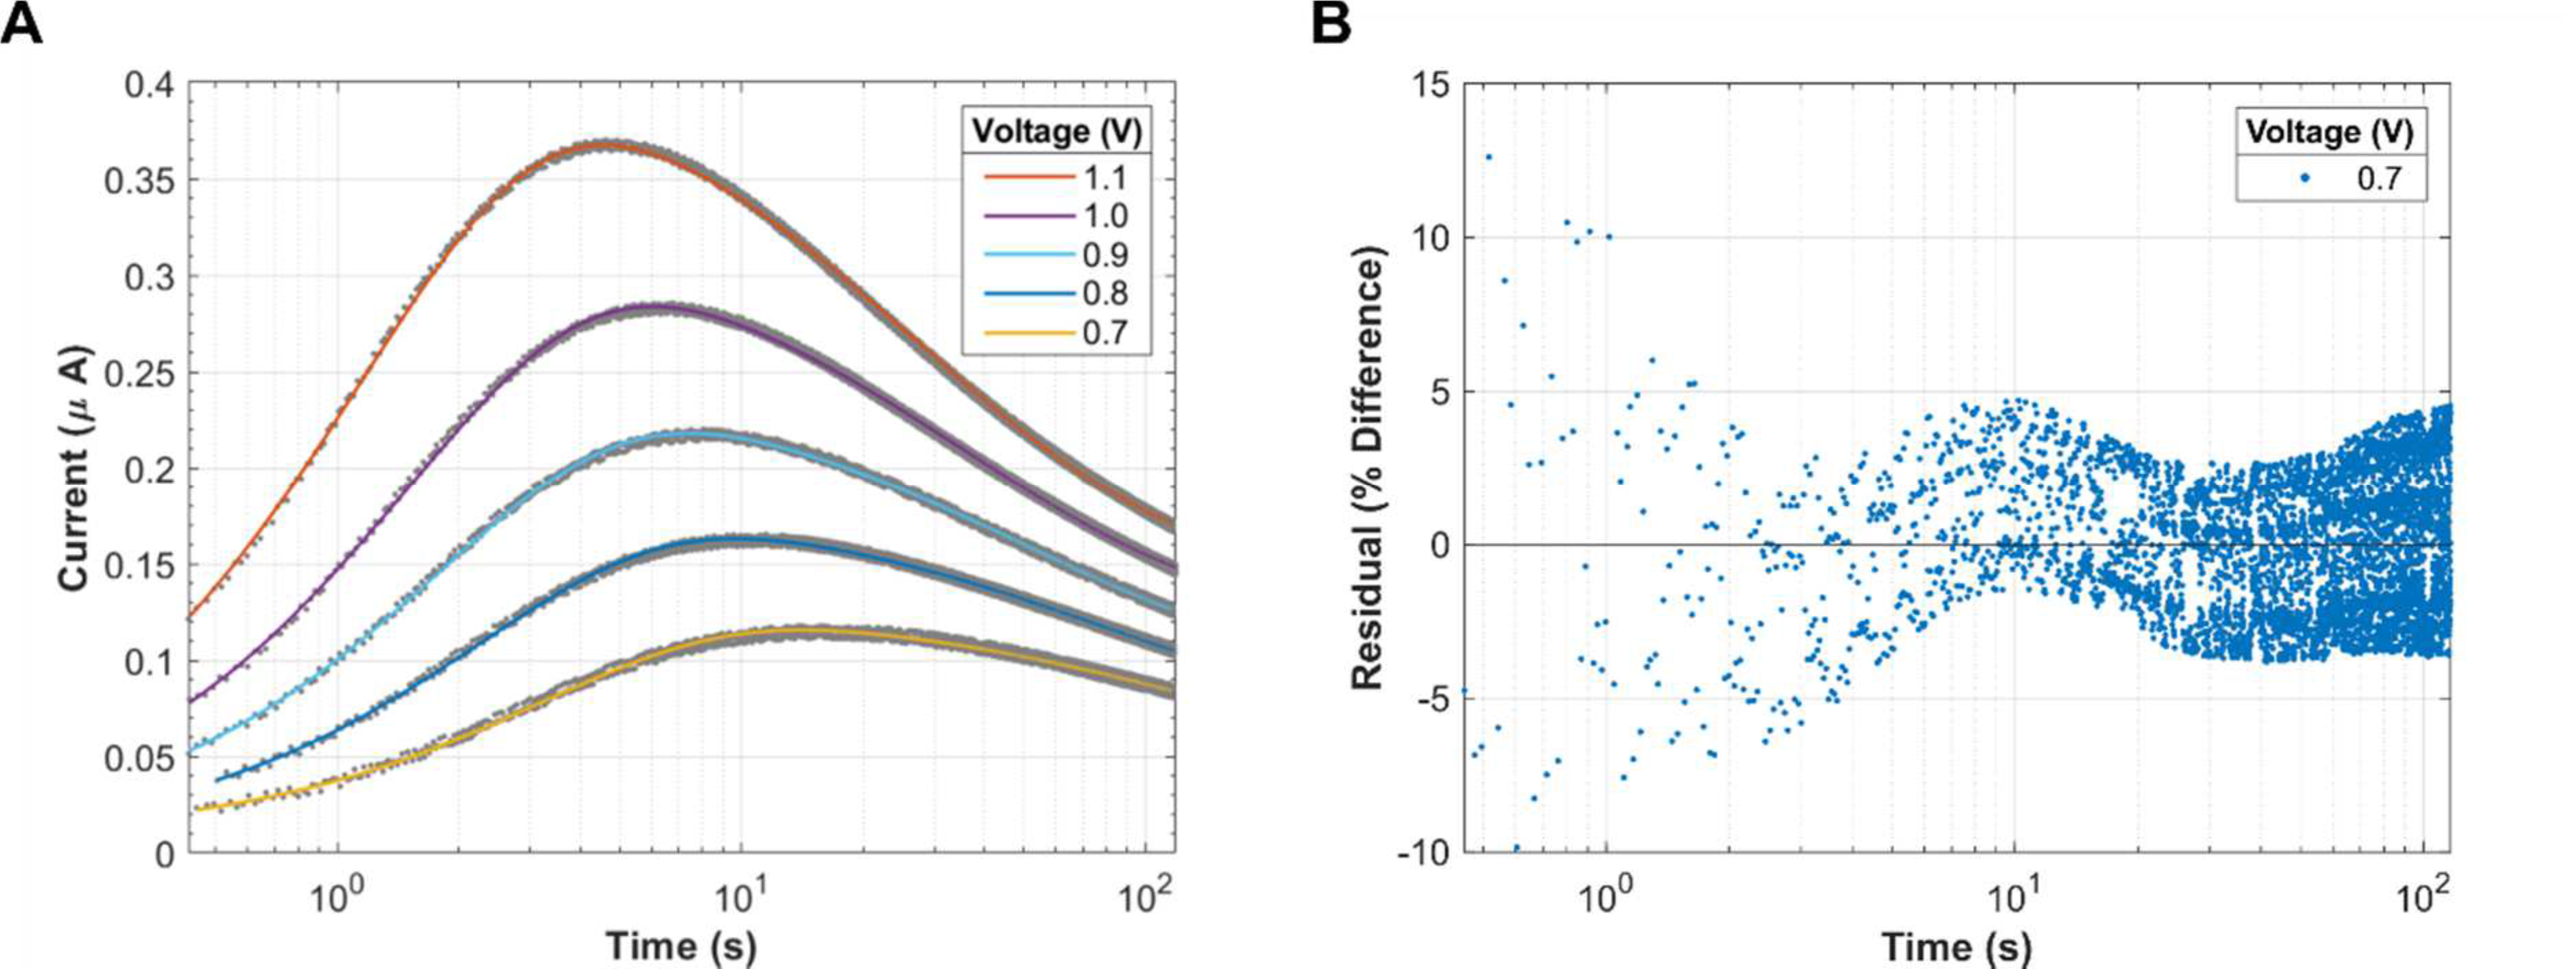
\includegraphics[width=0.7\textwidth]{Chapter6/Figs/e.png}
    \caption[A single layer of spiking neural network with RRAM synapses organized in crossbar architecture.]{A single layer of spiking neural network with RRAM synapses organized in crossbar architecture. Post-synaptic neuron connects with a pre-synaptic neuron with several RRAM synapses in parallel. Back-propagated spikes after dendritic processing modulate RRAM in-situ under STDP learning rule \cite{wu2018dendritic}.}
    \label{fig:6e}
\end{figure}

% \noindent The presented architectural configuration bears resemblance to existing memory architectures, wherein the devices are arranged in a dense two-dimensional array with the input and output neurons constituting the peripheral circuitry, laid out at a matching pitch with the memory array. This layout forms a repeatable motif that can be scaled to deeper SNN architectures.\\

% \noindent The extension of larger 3D IC architectures using through-silicon-via (TSVs) represents a natural pathway for further scaling to very high integration density and network complexity. This can be achieved without resorting to the overhead incurred by asynchronous communication protocols such as the address-event-representation (AER) \cite{jo2009programmable}.\\

\noindent The presented architectural configuration resembles existing memory architectures, where devices are arranged in a dense two-dimensional array with input and output neurons forming peripheral circuitry, laid out at a matching pitch with the memory array. This layout forms a repeatable motif scalable to deeper SNN architectures. Extending to larger 3D IC architectures using through-silicon-via (TSVs) represents a natural pathway for further scaling to very high integration density and network complexity. This can be achieved without the overhead of asynchronous communication protocols such as address-event-representation (AER) \cite{jo2009programmable}.\\

% \noindent It is desirable to have non-volatile analog-like weights in order to achieve effective STDP learning \cite{gaba2013stochastic}. However, the majority of practical \cite{soni2011stochastic}, small-sized RRAM devices exhibit abrupt switching behaviour \cite{yu2012switching}, which consequently limits the stable synaptic resolution to 1-bit (or binary, bistable) \cite{suri2013bio}. \\

% \noindent Furthermore, the switching probability and switching times of these devices typically depend upon the voltage applied across the device, as well as the duration of the voltage pulse \cite{li2014stochastic}. In order to circumvent the binary resolution of these devices, a compound memristive synapse with multiple bistable devices in parallel was previously proposed as a means of emulating analog weights on average \cite{bill2014compound}.\\

\noindent Non-volatile analog-like weights are desirable for effective STDP learning \cite{gaba2013stochastic}. However, most practical \cite{soni2011stochastic}, small-sized RRAM devices exhibit abrupt switching behavior \cite{yu2012switching}, which limits stable synaptic resolution to 1-bit (or binary, bistable) \cite{suri2013bio}.  Furthermore, device switching probability and times typically depend on the applied voltage and pulse duration \cite{li2014stochastic}. To circumvent binary resolution, a compound memristive synapse with multiple bistable devices in parallel was previously proposed to emulate analog weights on average \cite{bill2014compound}.\\

% \noindent Theoretical studies have demonstrated that the STDP learning rule facilitates unsupervised local learning in spiking neural networks through the implementation of a Bayesian expectation-maximisation algorithm \cite{nessler2013bayesian} and hidden Markov models \cite{kappel2014stdp}. Furthermore, a nonlinear STDP learning function, such as an exponentially shaped window observed in biological neural systems \cite{toyoizumi2004spike}, is essential for ensuring the stability and efficiency of the computing process \cite{sprekeler2007slowness}. \\

\noindent Theoretical studies have demonstrated that the STDP learning rule facilitates unsupervised local learning in spiking neural networks through implementing a Bayesian expectation-maximisation algorithm \cite{nessler2013bayesian} and hidden Markov models \cite{kappel2014stdp}. Furthermore, a nonlinear STDP learning function, such as an exponentially shaped window observed in biological neural systems \cite{toyoizumi2004spike}, is essential for ensuring the stability and efficiency of the computing process \cite{sprekeler2007slowness}.\\

% \noindent As previously stated, emerging memristive nanoscale devices are being considered as a means of enabling the realisation of large-scale neuromorphic hardware. Nanoscale implementations of memristors \cite{krzysteczko2012memristive}, including phase-change memory (PCM) \cite{kang2015emulation}, resistive random-access memory (RRAM) \cite{mandal2014novel}, and spin-torque-transfer random-access memory (STT-RAM) \cite{sengupta2015spin}, have been demonstrated to exhibit switching characteristics analogous to those observed in spike-timing-dependent plasticity (STDP) \cite{li2013ultrafast}.\\

% \noindent  These devices enable the highly desired advantage of a small silicon area of $4F^2$ (\textit{F} is the feature size of the semiconductor fabrication process) \cite{chen2016review}, ultra-energy-efficient operation of sub-pico-Joule per switching event, CMOS compatibility, and dense crossbar (or crosspoint) arrays and 3D integration.\\

\noindent As previously stated, emerging memristive nanoscale devices are being considered as a means of enabling the realization of large-scale neuromorphic hardware. Nanoscale implementations of memristors \cite{krzysteczko2012memristive}, including phase-change memory (PCM) \cite{kang2015emulation}, resistive random-access memory (RRAM) \cite{mandal2014novel}, and spin-torque-transfer random-access memory (STT-RAM) \cite{sengupta2015spin}, have been demonstrated to exhibit switching characteristics analogous to those observed in spike-timing-dependent plasticity (STDP) \cite{li2013ultrafast}. Furthermore, these devices offer the highly desired advantages of a small silicon area of $4F^2$ (\textit{F} is the feature size of the semiconductor fabrication process) \cite{chen2016review}, ultra-energy-efficient operation of sub-pico-Joule per switching event, CMOS compatibility, and dense crossbar (or crosspoint) arrays and 3D integration.\\

\begin{figure}[htbp!] 
    \centering    
    \includegraphics[width=0.65\textwidth]{Chapter6/Figs/f.png}
    \caption[A pair of spikes are applied across a synapse to create relative-timing dependent net potential.]{A pair of spikes are applied across a synapse to create relative-timing dependent net potential $V_{net}$, of which the over-threshold portion $V_{eff}$ may cause the RRAM resistance to switch \cite{wu2017enabling}.}
    \label{fig:6f}
\end{figure}

\noindent In particular, RRAM devices exhibit characteristics that are analogous to those of biological synapses. Furthermore, RRAMs exhibit conductance levels comparable to synaptic strength (or weight), and their conductance can be modified by voltage pulses. Notably, RRAMs are capable of directly implementing spike-timing-dependent plasticity (STDP) through identical pair-wise spikes As illustrated in Figure \ref{fig:6f}, the net potential $V_{net}$ created by a pre-synaptic spike and a late arriving post-synaptic spike, with $t > 0$, produces an over-threshold, $V_{th}^+$, portion $V_{eff}$, which then causes an increase in conductance in a typical RRAM. Conversely, a presynaptic spike and an earlier arriving post-synaptic spike with $t < 0$ produces $V_{eff}$ that crosses the negative threshold, $V_{th}^-$, and thus causes a decrease in the conductance. \\

% \noindent A memristor with analogue resistance is an optimal choice for STDP learning. However, experimental studies indicate that the majority of nanoscale implementations of memristive RRAMs exhibit a stochastic process in their filament formation, as well as an abrupt conductance change once the filament is formed \cite{prakash2016multilevel}. The results demonstrate an abrupt transition from the high resistance state (HRS) to the low resistance state (LRS), as well as notable variations in the switching threshold voltages and HRS/LRS transitions, which tend to be stochastic in nature.\\

\noindent A memristor with analogue resistance is an optimal choice for STDP learning. However, experimental studies indicate that most nanoscale implementations of memristive RRAMs exhibit a stochastic process in their filament formation, as well as an abrupt conductance change once the filament is formed \cite{prakash2016multilevel}. The results demonstrate an abrupt transition from the high resistance state (HRS) to the low resistance state (LRS), as well as notable variations in switching threshold voltages and HRS/LRS transitions, which tend to be stochastic.\\

% \noindent The intrinsic stochastic switching in RRAM therefore limits the stable synaptic resolution to 1 bit, or bistable behaviour. In order to unlock STDP-based learning in SNN hardware, a solution enabling non-linear, especially exponential, STDP learning functions with binary RRAMs is therefore highly desirable. \\

% \noindent One proposed approach to enable the complexity of learnable tasks to be scaled up in fully MSNNs by directly applying gradient descent to the nonlinear state evolution of memristive neurons and synapses \cite{zhou2022memristive}. The modelling of both neurons and synapses in biological neural networks employs the use of memristors. The MIF neuron model has been devised with the objective of achieving distinct depolarisation, hyperpolarisation and repolarisation voltage phases with a minimal set of circuit elements. \\

\noindent The intrinsic stochastic switching in RRAM therefore limits stable synaptic resolution to 1 bit, or bistable behavior. To enable STDP-based learning in SNN hardware, a solution for non-linear, especially exponential, STDP learning functions with binary RRAMs is highly desirable. One proposed approach to scale up the complexity of learnable tasks in fully MSNNs is by directly applying gradient descent to the nonlinear state evolution of memristive neurons and synapses \cite{zhou2022memristive}. Modelling of both neurons and synapses in biological neural networks employs memristors. The MIF neuron model has been devised to achieve distinct depolarisation, hyperpolarisation, and repolarisation voltage phases with a minimal set of circuit elements.\\

% \noindent Memristive synapses serve as interconnects between layers of neurons. This allows for the development of dynamical, time-varying memristive neurons, which are capable of learning and achieving significantly enhanced accuracy on data-driven tasks compared to previous reports on MSNNs \cite{neftci2019surrogate}. By leveraging the analog spiking characteristics inherent to the MIF neuron model, the non-differentiability of spike-based activations is entirely circumvented.\\

\noindent Memristive synapses serve as interconnects between layers of neurons. This allows for the development of dynamical, time-varying memristive neurons, capable of learning and achieving significantly enhanced accuracy on data-driven tasks compared to previous reports on MSNNs \cite{neftci2019surrogate}. By leveraging the analog spiking characteristics inherent to the MIF neuron model, the non-differentiability of spike-based activations is entirely circumvented.\\

% \noindent In order to account for the hardware implementation of a fully MSNN, it is necessary to consider the voltage response of the MIF neuron, which must drive the memristive synapses. The synaptic conductances are correspondingly weighted by this response. This can be fully integrated into a crossbar according to the following equation:

\noindent To account for the hardware implementation of a fully MSNN, it is necessary to consider the MIF neuron's voltage response, which must drive the memristive synapses. The synaptic conductances are correspondingly weighted by this response. This can be fully integrated into a crossbar according to the following equation:
\begin{align}
\begin{matrix}
& \textbf{G} & \\
& \begin{bmatrix}
    w_{1,1} & w_{1,2} & \cdots & w_{1, m} \\
    w_{2,1} & w_{2,2} & \cdots & w_{2, m} \\
    \vdots & \vdots & \vdots & \vdots \\
    w_{n, 1} & w_{n, 2} & \cdots & w_{n, m}
\end{bmatrix} &\\
\end{matrix}
\begin{matrix}
  & \textbf{V} & \\
 & \begin{bmatrix}
V_{1} \\
V_{2} \\
\vdots \\
V_{n}
\end{bmatrix} &\\
\end{matrix}
\begin{matrix}
 & = & \\
\\
\\
&=&  \\
\\
\end{matrix}
\begin{matrix}
  & \textbf{I} & \\
 & \begin{bmatrix}
I_{1} \\
I_{2} \\
\vdots \\
I_{m}
\end{bmatrix} &\\
\end{matrix}
\label{eq:6.18}
\end{align}


\noindent where \textbf{\textit{I}} is the output current vector, \textbf{\textit{V}} is the input voltage vector, and \textbf{\textit{G}} is the conductance matrix of the crossbar.
\begin{align}
I_n = \sum_{i=1}^{m} v_i \cdot w_{n,i} \label{eq:6.19}
\end{align}

\noindent The output current vector is generated via bitline current summation, as illustrated in equation (\ref{eq:6.19}), and is directly driven into the input of the subsequent MIF neuron layer. Resistive loading may result in the attenuation of the output current in subsequent stages \cite{wang2020high}; however, this can be accounted for through the utilisation of a scaling factor or the implementation of a buffer \cite{wang2022low}.
\begin{align}
\tau_{syn} \frac{dI}{dt} &= a - I \label{eq:6.20} \\
\tau_{syn}\frac{da}{dt} &= W_i \cdot\sum_{n}\delta\left( t - t_i^n \right) \label{eq:6.21}
\end{align}

\noindent A considerable number of neural coding studies portray spike trains as a superposition of time-shifted Dirac delta pulses, represented by $\sum_{n}\delta\left( t - t_i^n \right)$. Consequently, this model of spikes is one idealisation. The spike train is employed to modulate a time-continuous alpha input current \textit{I}, which has been modelled by the differential equation (\ref{eq:6.20}) presented in order to ensure compatibility with real, physical systems. \\

\noindent In this series of equations (\ref{eq:6.21}), \textit{a} represents an internal state variable, which often corresponds to physical quantities such as the concentration of oxygen vacancies or the length of filaments in resistive switching materials, $\tau_{syn}$ denotes a time constant that determines the shape of the alpha current, and $W_i$ is the synaptic weight between a presynaptic neuron \textit{i} and its associated postsynaptic neuron. It is widely accepted that such alpha waveforms correspond to the response from biological neurons in the sensory periphery that respond with graded potentials \cite{eshraghian2018formulation}.
\begin{align}
I^{t+1} &=  I^t + \frac{a^t - I^t}{\tau_{syn}} \label{eq:6.22} \\
a^{t+1} &= a^t - \frac{a^t}{\tau_{syn}} + \sum_{n}\delta\left( t - t_i^n \right)\label{eq:6.23}
\end{align}


% \noindent In order to train a network of MIF neurons and synapses using gradient descent, the differential equations representing the MIF circuit dynamics are recast into discrete-time form (\ref{eq:6.22}, \ref{eq:6.23}). This allows the memristive dynamics to be captured in a computational graph that evolves over time, in a manner analogous to that of a recurrent neural network (RNN).\\

% \noindent In practice, SPICE-like simulators employ a variety of differential equation solvers, including the backward Euler method and the fourth-order Runge-Kutta method (RK4). In order to ensure compatibility with the BPTT algorithm, the differential equations are solved using the forward Euler method, which provides an explicit representation of the next time step based on present-time dynamics. \\

\noindent To train a network of MIF neurons and synapses using gradient descent, the differential equations representing the MIF circuit dynamics are recast into discrete-time form (\ref{eq:6.19}, \ref{eq:6.20}). This allows memristive dynamics to be captured in a computational graph that evolves over time, analogous to a recurrent neural network (RNN). In practice, SPICE-like simulators employ various differential equation solvers, including the backward Euler method and the fourth-order Runge-Kutta method (RK4). To ensure compatibility with the BPTT algorithm, the differential equations are solved using the forward Euler method, providing an explicit representation of the next time step based on present-time dynamics. \\

% \noindent The intricate dynamics of the MIF neuronal network are now accounted for in the MSNN, which is unrolled in time in such a way that gradient descent can be used to optimise the memristive synapses as a function of the MIF evolution. The discrete-time solution can be illustrated as a directed, acyclic graph, where time flows in one direction. \\

% \noindent In order to train a network, a loss function is calculated using the membrane potential \textit{v} of the output layer at each step. It should be noted that the adjoint method \cite{chen2018neural} is normally not adopted, as an intermediate state is required in order to calculate the loss and guide the training process for each time step. The focus is on the spiking output at all time steps, rather than just on the final state of the system, which makes BPTT a more optimal choice.\\

\noindent The intricate dynamics of the MIF neuronal network are now accounted for in the MSNN, which is unrolled in time such that gradient descent can optimize the memristive synapses as a function of the MIF evolution. The discrete-time solution can be illustrated as a directed, acyclic graph, where time flows in one direction. To train a network, a loss function is calculated using the membrane potential \textit{v} of the output layer at each step. It should be noted that the adjoint method \cite{chen2018neural} is normally not adopted, as an intermediate state is required to calculate the loss and guide the training process for each time step. The focus is on the spiking output at all time steps, rather than just the final system state, making BPTT a more optimal choice.\\

% \noindent The predicted MIF neuron is expected to spike most frequently by aiming to increase the membrane potential across time steps, while the incorrect target should be suppressed. Given that the membrane dynamics are continuous, it is possible to train a fully analogue MSNN, as has become the norm in the training of deep SNNs via error backpropagation \cite{neftci2019surrogate}.\\

% \noindent The BPTT algorithm employs an iterative application of the chain rule from the output back to the leaf nodes in order to determine the optimal update direction for the network \cite{eshraghian2023training}, with previous demonstrations have treated \textit{w} as the device conductance. This approach offers a more biorealistic representation and can be fully integrated using RRAM crossbars.

\noindent The predicted MIF neuron is expected to spike most frequently by aiming to increase the membrane potential across time steps, while the incorrect target should be suppressed. Given that membrane dynamics are continuous, it is possible to train a fully analogue MSNN, as has become the norm in training deep SNNs via error backpropagation \cite{neftci2019surrogate}. The BPTT algorithm employs iterative application of the chain rule from the output back to the leaf nodes to determine the optimal update direction for the network \cite{eshraghian2023training}, with previous demonstrations treating w as the device conductance. This approach offers a more biorealistic representation and can be fully integrated using RRAM crossbars.

\subsection[Conductance Mapping]{Conductance Mapping}


% The approaches described in the preceding sections pertained to memristive neural networks (MNNs) that had been trained through conventional methodologies without consideration of the non-idealities. The primary challenge lies in the discrepancy between the behaviour of conventional SNNs and that of MNNs. \\

% \noindent The synapses of the former typically exhibit a consistent response and typically relate inputs to outputs in a linear fashion. In contrast, MNNs utilise synapses implemented using memristors, which can become fixed in a particular state, exhibit varying responses over time, due retention or random telegraph noise (RTN), and even produce nonlinear outputs, I-V nonlinearity. \\

\noindent The approaches described in the preceding sections pertained to memristive neural networks (MNNs) trained through conventional methodologies without considering non-idealities. The primary challenge lies in the discrepancy between conventional SNNs and MNNs. The former's synapses typically exhibit consistent, often linear, responses. In contrast, MNNs utilize memristor-implemented synapses, which can become fixed in a particular state, exhibit varying responses over time due to retention or random telegraph noise (RTN), and even produce nonlinear outputs (I-V nonlinearity).\\

% \noindent A substantial proportion of the literature on addressing memristor nonidealities focuses on modifications at the hardware level. These may entail: Modifications to the device structure are a common approach, as evidenced by the literature \cite{fang2018improvement}; additional circuitry is another avenue of exploration \cite{ambrogio2018equivalent, li2018analogue}; programming and mapping schemes are also subject to modification \cite{xia2017stuck}; in-situ retraining is a further strategy, as exemplified by the literature \cite{chen2017accelerator, jain2019cxdnn, wang2020ssm, li2019build}.\\

% \noindent However, these techniques may have some drawbacks. For example, pulse-width modulation \cite{amirsoleimani2020memory}, may minimise the effects of I-V nonlinearities; however, this comes at the cost of increased clock cycles \cite{cai2019fully}. Furthermore, hardware-level changes are often technology-specific, thus rendering them difficult to apply to a wide range of device types.\\

\noindent A substantial proportion of the literature addressing memristor nonidealities focuses on hardware-level modifications. These may entail: modifications to the device structure \cite{fang2018improvement}; additional circuitry \cite{ambrogio2018equivalent, li2018analogue}; programming and mapping schemes \cite{xia2017stuck}; and in-situ retraining \cite{chen2017accelerator, jain2019cxdnn, wang2020ssm, li2019build}. However, these techniques may have drawbacks. For example, pulse-width modulation \cite{amirsoleimani2020memory} may minimize I-V nonlinearities at the cost of increased clock cycles \cite{cai2019fully}. Furthermore, hardware-level changes are often technology-specific, hindering broad applicability.\\

% \noindent As an alternative, techniques that do not interfere with the hardware, such as committee machines (CMs), may be employed. These allow the performance of MNNs to be improved by combining them and require only the average of the outputs of crossbar arrays \cite{joksas2020committee}. Additionally, modifications to ex situ training have been previously proposed. \\

% \noindent Common approaches include adjusting the loss function \cite{zhu2020statistical} or introducing noise into the synaptic weights \cite{he2019noise} or conductances that implement those synaptic weights \cite{joshi2020accurate}, thereby enhancing the resilience of MNNs to the effects of non-idealities. It is evident that ex situ training represents a promising methodology for enhancing the feasibility of MNNs.\\

\noindent As an alternative, techniques that do not interfere with hardware, such as committee machines (CMs), may be employed. These improve MNN performance by combining them and require only the average of crossbar array outputs \cite{joksas2020committee}. Additionally, modifications to ex situ training have been previously proposed. Common approaches include adjusting the loss function \cite{zhu2020statistical} or introducing noise into synaptic weights \cite{he2019noise} or conductances that implement those weights \cite{joshi2020accurate}, thereby enhancing MNN resilience to non-idealities. It is evident that ex situ training represents a promising methodology for enhancing MNN feasibility.\\

% \noindent However, previous approaches have only considered a limited number of non-idealities. For example, injection of noise into the conductances is insufficient in many situations, as the effect of non-idealities such as I-V nonlinearity cannot be represented by the disturbance of the weights alone. Furthermore, conventional weight implementations do not map naturally to resistive crossbar arrays, while training validation schemes are not well suited to the often stochastic nature of MNNs.\\

% \noindent This research focuses on enhancing the efficacy of \textit{ex-situ} training of memristive SNNs, while also evaluating the resilience of this approach. To this end, data from a $SiO_x$ memristive device is employed, complemented by insights drawn from existing literature.\\

\noindent However, previous approaches have considered only a limited number of non-idealities. For example, injecting noise into conductances is insufficient in many situations, as the effect of non-idealities like I-V nonlinearity cannot be represented solely by weight disturbance. Furthermore, conventional weight implementations do not map naturally to resistive crossbar arrays, while training validation schemes are not well suited to the often stochastic nature of MNNs. This research focuses on enhancing the efficacy of \textit{ex-situ} training of memristive SNNs, while also evaluating this approach's resilience. To this end, data from a  $SiO_x$  memristive device is employed, complemented by insights from existing literature.\\

\begin{figure}[htbp!] 
\centering    
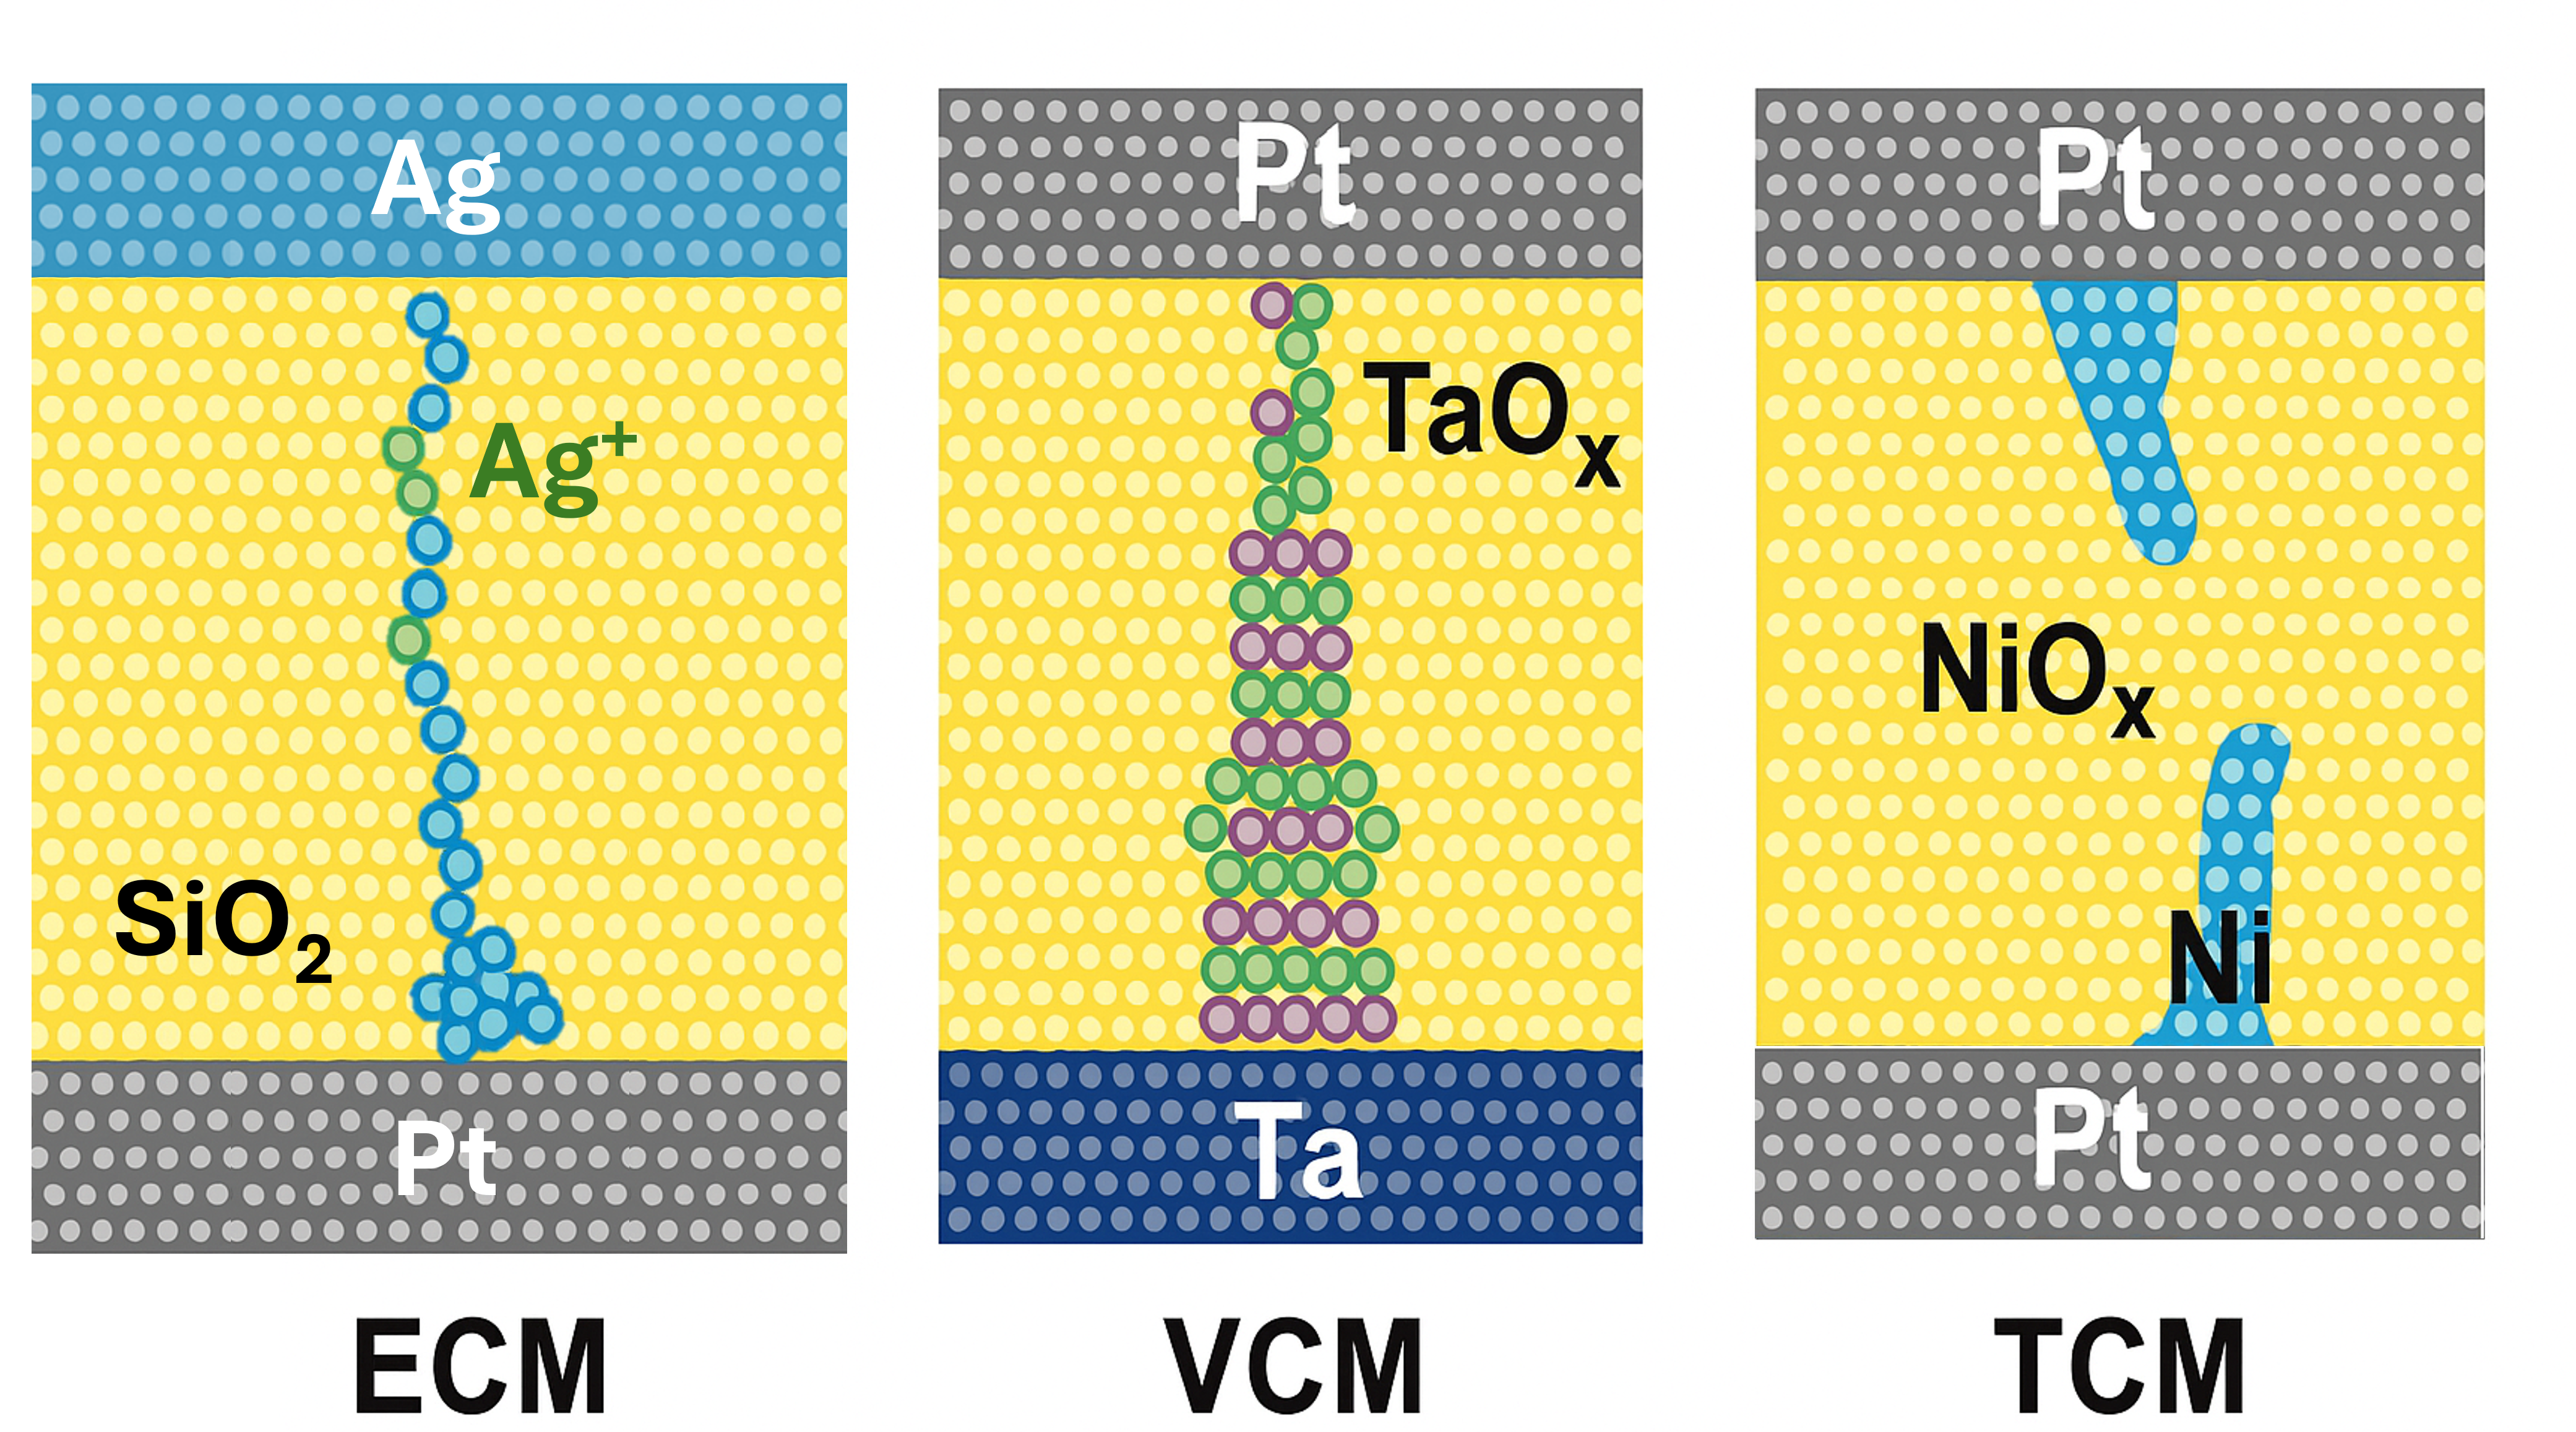
\includegraphics[width=1\textwidth]{Chapter6/Figs/g.png}
\caption[Single sweeps of 53 resistance states of a $SiO_x$ device.]{Single sweeps of 53 resistance states of a $SiO_x$ device. Different states were obtained by incrementing maximum voltage by 0.05V. Every seventh state shares the same colour; this does not indicate any other relationship between such states \cite{Barmpatsalos2021-yn}.}
\label{fig:6g}
\end{figure}


\noindent The $SiO_x$ resistive random-access memory (RRAM) device comprised a $1 \mu m Si/SiO_2$  switching layer positioned between a 100nm $Mo$ bottom electrode and a 100nm $Au$ top electrode. Furthermore, a 5nm $Ti$ wetting layer was incorporated between the $SiO_x$ and $Au$ electrodes. Following electroforming and additional validation procedures, positive sweeps were conducted on the $SiO_x$ device, commencing from 0.5V and increasing by 0.05V in each run, thereby generating resistance states that spanned multiple orders of magnitude.\\

% \noindent The majority of existing literature on ex-situ training of MNNs assumes a linear relationship between inputs and outputs at the level of individual devices. Non-linearities are only introduced at the level of the activation functions. In particular, outputs are assumed to be a function of the product of a vector of applied inputs and a matrix of weights:
\noindent Most existing literature on ex-situ training of MNNs assumes a linear relationship between inputs and outputs at the individual device level, with nonlinearities introduced only at the activation function level. Specifically, outputs are assumed to be a function of the product of an applied input vector and a weight matrix:
\begin{align}
y_j = f\left( \sum_{i=1}^{M} x_i, w_{ij} \right) \label{eq:6.24}
\end{align}


\noindent Where the outputs, $y_j \in \textbf{y} \in \mathbb{R}^{1 \times N}$ is calculated using the inputs $x_i \in \textbf{x} \in \mathbb{R}^{1 \times M}$, weights $w_{ij} \in \textbf{w} \in \mathbb{R}^{M \times N}$, and a nonlinear activation function $f$. Non-Ohmic behaviour manifests itself in individual devices only, therefore these nonlinear effects can be separated from the other devices. To take I-V nonlinearities into account in ex-situ MNN training, the products in (\ref{eq:6.24}) can be replaced with a nonlinear function to give:
\begin{align}
y_j = f\left( \sum_{i=1}^{M} g \left( x_i, w_{ij} \right) \right) \label{eq:6.25}
\end{align}

% \noindent In order to account for the non-ohmic behaviour of memristors, Function \textit{g} must be modified to reflect the specific characteristics of the mapping scheme between weights and conductances, as well as the non-ohmic device behaviour model, which is typically dependent on the type of devices employed \cite{joksas2022nonideality}.\\

\noindent To account for memristor non-ohmic behavior, Function \textit{g} must be modified to reflect the specific characteristics of the mapping scheme between weights and conductances, as well as the non-ohmic device behavior model, which typically depends on the device type employed \cite{joksas2022nonideality}.\\

% \noindent The mapping scheme that relates weights and conductances is a crucial aspect to consider when designing memristive neural networks. In typical artificial neural networks, synaptic weights can assume any real value. Conversely, conductances are constrained to be non-negative.\\

% \noindent To address this discrepancy, a neural network architecture was devised whereby twice the number of weights are trained, but each is constrained to be non-negative. This enables the association of weights with the conductances of individual devices, thereby creating a more natural mapping and facilitating adaptation to non-idealities. Additionally, it allows for more precise control over power consumption.\\

\noindent The mapping scheme relating weights and conductances is a crucial aspect in designing memristive neural networks. In typical artificial neural networks, synaptic weights can assume any real value. Conversely, conductances are constrained to be non-negative. To address this discrepancy, a neural network architecture was devised where twice the number of weights are trained, but each is constrained to be non-negative. This enables the association of weights with individual device conductances, creating a more natural mapping and facilitating adaptation to non-idealities. Additionally, it allows for more precise control over power consumption.\\

\noindent The aforementioned mappings are performed in an identical manner in the specific instance of fully connected synaptic layers in artificial neural networks, provided that conventional weight implementation methodologies are utilised. Both the inputs, designated as $x \in \mathbf{x}$, and the outputs, represented by $y \in \mathbf{y}$, are mapped onto voltages \textit{V} and total output currents \textit{I}, using the scaling factors $k_V$ and $k_I$, where $k_G$ is the conductance scaling factor:
\begin{align}
V &= k_V x \label{eq:6.26} \\
y &= \frac{I}{k_I} = \frac{I}{k_V k_G} \label{eq:6.27} \\
k_G &= \frac{G_{max} - G_{min}}{max |\mathbf{W}|} = \frac{G_{on} - G_{off}}{max |\mathbf{W}|}\label{eq:6.28}
\end{align}


\noindent  Irrespective of the scheme employed, a minimum of two conductances are required to encode both positive and negative weights. Conductances $G_+$ and $G_-$ are introduced into the "positive" and "negative" bit lines of the differential pair architecture, respectively. The proportionality of each weight is determined by the difference $G_+ - G_-$, with $k_G$ serving as the constant of proportionality. This enables the encoding of any real number within a finite range. In a typical differential pair implementation, $G_{min} = G_{off}$ and $G_{max} = G_{on}$. In an alternate proportional mapping scheme, $G_{min} = 0$ and $G_{max} = G_{on}$ to give $k_G = \frac{g_{on}}{max |\mathbf{W}|}$.\\

\noindent The issues associated with proportional mapping schemes, such as unimplementable regions, are not the only obstacles. Conventional differential pair realization also presents design challenges. For example, infinite conductance combinations will produce the same difference \cite{kim20214k}, i.e., the same effective conductance. This implies an arbitrary choice may be necessary for mapping weights to conductances. To illustrate, consider encoding weights $W \in \mathbf{W}$. In this case, pairs of conductances $G_+$ and $G_-$ may be picked symmetrically around the average value:
\begin{align}
G\pm &= G_{avg} \pm \frac{k_G w}{2} \label{eq:6.29} \\
G_{avg} &= \frac{G_{off} + G_{on}}{2} \label{eq:6.30}
\end{align}


% \noindent While multiple mapping schemes may yield the same conductance difference, some may prove more advantageous than others. The scheme in (\ref{eq:6.29}) can be beneficial in certain scenarios, as it typically reduces the number of conductances near $G_{off}$ and $G_{on}$, which are often more challenging to achieve. However, the selection of the mapping scheme can be explicitly linked to specific objectives.\\

\noindent While multiple mapping schemes may yield the same conductance difference, some may prove more advantageous. The scheme in (\ref{eq:6.26}) can be beneficial in certain scenarios, as it typically reduces the number of conductances near $G_{off}$ and $G_{on}$, which are often more challenging to achieve. However, mapping scheme selection can be explicitly linked to specific objectives.\\

% \noindent The differential pair architecture can be employed to mitigate the effects of stuck devices. To illustrate, if $G_+$ is stuck in an undesirable state, $G_-$ can be adjusted to minimise the negative effects. An alternative approach is to employ a simpler scheme that optimises a specific metric, such as power consumption. \\

% \noindent This is illustrated in the simulations presented in this chapter, where conventional weights are used. In these simulations, a scheme that minimises power consumption is employed by ensuring that at least one of ${G_+, G_-}$ is set to $G_{off}$:
\noindent The differential pair architecture can mitigate the effects of stuck devices. For instance, if $G_+$ is stuck in an undesirable state, $G_-$ can be adjusted to minimize negative effects. An alternative approach is to employ a simpler scheme that optimizes a specific metric, such as power consumption. This is illustrated in the simulations in this chapter, where conventional weights are used. In these simulations, a scheme minimizing power consumption is employed by ensuring at least one of ${G_+, G_-}$ is set to $G_{off}$:
\begin{align}
G_+ &= G_{off} + max\left\{ 0, k_GW \right\} \label{eq:6.31} \\
G_- &= G_{off} - min\left\{ 0, k_GW \right\} \label{eq:6.32}
\end{align}

\noindent An alternative approach is to utilise two sets of non-negative weights, $W^+_{ij} \in \mathbf{W}_+ \in \mathbb{R}^{M \times N}_{\ge 0}$ and $W^-_{ij} \in \mathbf{W}_+ \in \mathbb{R}^{M \times N}_{\ge 0}$, which are collectively referred to as double weights \cite{kendall2020training}. This method entails mapping each weight onto a single conductance in the aforementioned "positive" and "negative" bit lines, respectively. \\

\noindent Despite the nonnegativity of each weight, the differential pair architecture allows for encoding the negative contribution of the $i_{th}$ input on the $j_{th}$ output through the introduction of a subtraction operation in hardware. Only the nonlinearity-aware node function in (\ref{eq:6.25}) requires adjustment to give:
\begin{align}
y_j = f\left( \sum_{i=1}^{M} g\left( x_i,W_{i,j}^+ \right) - g\left( x_i,W_{i,j}^- \right) \right) \label{eq:6.33}
\end{align}

\noindent As all weights in $\mathbf{W} := [W_+, W_-]$ are non-negative, they can be related to the corresponding conductances in the same way: $W_{\pm} \in [0, max(\mathbf{W})]$ can be linearly mapped onto $G_{\pm} \in [G_{off}, G_{on}]$, thus avoiding the introduction of weight gaps:
\begin{align}
G_{\pm} = k_GW_{\pm} + G_{off} \label{eq:6.34}
\end{align}

% \noindent The initial benefit of utilising double weights is that the conductances are more directly exposed to the training algorithm. This enables the selection of combinations that achieve both optimal performance, for example in terms of loss and robustness. To illustrate, if specific non-idealities manifest more at lower conductance values, such as with programming deviations \cite{kim2016voltage}, the training may be able to select pairs at higher values, while maintaining the same difference between $G_+$ and $G_-$. This allows the minimisation of the negative effects of non-idealities without the need to explicitly specify which conductance pairs should be selected. \\

\noindent The initial benefit of utilizing double weights is that conductances are more directly exposed to the training algorithm, enabling selection of combinations that achieve optimal performance (e.g., loss and robustness). To illustrate, if specific non-idealities manifest more at lower conductance values (e.g., programming deviations \cite{kim2016voltage}), training may select pairs at higher values while maintaining the same $G_+$ and $G_-$ difference, minimizing negative non-ideality effects without explicit specification of conductance pairs.

\section{Inference and Classification}

% In the context of spiking neural networks (SNNs), neurons facilitate the exchange of information through the emission of spikes. This phenomenon represents a neural network architecture predicated on individual spikes \cite{liu2014memristor}. The SNN architecture is therefore structurally analogous to the human brain. \\

% \noindent The signal in SNNs can utilise both pulse coding and rate coding, and permits multiplexing of information as frequency and amplitude. In certain forms of electronic SNNs, spikes exhibit a waveform shape that is analogous to that of biological spikes. However, in general electronic systems, spikes are represented in a far more simplified manner, typically by means of a square or Gaussian digital pulse. \\

% \noindent In SNN, the presence and timing of individual spikes are considered to be the means of communication and neural computation. The fundamental principle in the field of biology asserts that the greater the intensity of the input, the earlier the spike transmission occurs. Therefore, it is possible to design a network of spiking neurons with input neurons whose firing times are determined by an external stimulus \cite{serrano2013stdp}.

In spiking neural networks (SNNs), neurons facilitate information exchange through spike emission. This phenomenon represents a neural network architecture predicated on individual spikes \cite{liu2014memristor}. The SNN architecture is thus structurally analogous to the human brain. Signals in SNNs can utilize both pulse coding and rate coding, permitting multiplexing of information as frequency and amplitude. In certain electronic SNN forms, spikes exhibit a waveform shape analogous to biological spikes. However, in general electronic systems, spikes are represented in a far more simplified manner, typically as a square or Gaussian digital pulse.\\

\noindent In SNNs, the presence and timing of individual spikes are considered the means of communication and neural computation. The fundamental biological principle asserts that greater input intensity leads to earlier spike transmission. Therefore, it is possible to design a network of spiking neurons with input neurons whose firing times are determined by an external stimulus \cite{serrano2013stdp}.

\subsection[Nonidealities Calibrations]{Nonidealities Calibrations}

% In the simulation presented in this chapter, a combination of experimental data from a $SiO_x$ device, models based on simplified assumptions regarding breaking-down devices, and findings from the literature on programming variability were employed. I-V nonlinearities have been identified as a prevalent method for characterising deviations from ohmic behaviour in memristive devices.
\noindent In the simulation presented in this chapter, a combination of experimental data from a $SiO_x$ device, models based on simplified assumptions regarding breaking-down devices, and findings from the literature on programming variability were employed. I-V nonlinearities have been identified as a prevalent method for characterizing deviations from ohmic behavior in memristive devices.
\begin{align}
\gamma \equiv \frac{G\left( 2V_{ref} \right)}{G\left( V_{ref} \right)}  \label{eq:6.35}
\end{align}

% \noindent This approach involves the examination of two points on an I-V curve \cite{lentz2013current}, as previously discussed (\ref{eq:6.35}). This equation defines conductance linearity, which serves as a means of quantifying nonlinear I-V behaviour. A conductance linearity value of 1 is indicative of ohmic behaviour, while any deviation from this value indicates I-V nonlinearity. While this metric can be useful for describing non-ohmic behaviour at different voltages, it is more challenging to utilise for modelling purposes \cite{sung2018effect}.

\noindent This approach involves examining two points on an I-V curve \cite{lentz2013current}, as previously discussed (\ref{eq:6.32}). This equation defines conductance linearity, quantifying nonlinear I-V behavior. A conductance linearity of 1 indicates ohmic behavior; any deviation indicates I-V nonlinearity. While useful for describing non-ohmic behavior at different voltages, it is more challenging for modeling purposes \cite{sung2018effect}.
\begin{align}
I & = V_{ref}G\left ( \frac{V}{V_{ref}} \right )^{log_2 \gamma} \label{eq:6.36}
\end{align}

% \noindent In order to construct an I-V curve from a given nonlinearity parameter $\gamma$, it is possible to assume that the equality in Equation (\ref{eq:6.35}) holds for all $V$, rather than just $V_{ref}$. This would result in a relationship between current and voltage, as shown in (\ref{eq:6.35}). In this equation, $G$ represents the conductance parameter, which has a specific meaning in the context of $V_{ref}$, where the device produces the expected ohmic amount of current, which is equal to $V_{ref} G$.\\

\noindent To construct an I-V curve from a given nonlinearity parameter $\gamma$, it is possible to assume that the equality in Equation (\ref{eq:6.32}) holds for all $V$, rather than just $V_{ref}$. This would result in a relationship between current and voltage, as shown in (\ref{eq:6.32}). In this equation, $G$ represents the conductance parameter, which has a specific meaning in the context of $V_{ref}$, where the device produces the expected ohmic amount of current, equal to $V_{ref} G$.\\

\begin{figure}[htbp!] 
\centering    
\includegraphics[width=1\textwidth]{Chapter6/Figs/h.png}
\caption[I-V sweeps of a SiOx device are presented for two regions]{I-V sweeps of a SiOx device are presented for two regions: a) low-resistance region with average resistance ranging from 284.6 $\Omega$ to 1003 $\Omega$, and b) high-resistance region with average resistance ranging from 366.2 k$\Omega$ to 1.295 M$\Omega$. Only the voltage range from 0.0 V to 0.5 V was considered for all curves. The nonlinearity parameter was calculated by dividing the current at 0.5 V by the current at 0.25 V \cite{joksas2022nonideality}.}
\label{fig:6h}
\end{figure}

% \noindent The nonlinearity parameters $\gamma$ were extracted from experimental data obtained from a $SiO_x$ RRAM device. $SiO_x$ devices are capable of undergoing resistance switching, which is characterised by a typical I-V switching curve. In order to achieve a wide range of resistance states and to analyse I-V nonlinearity, incremental positive sweeps were employed to gradually reset the device from the low-resistance state (LRS) to the high-resistance state (HRS). The low-resistance discrete states display greater linearity and exhibit minimal variability. Conversely, the high-resistance states are more nonlinear, and the nonlinearity is less predictable.\\

\noindent Nonlinearity parameters $\gamma$ were extracted from experimental data obtained from a $SiO_x$  RRAM device. $SiO_x$ devices are capable of resistance switching, characterized by a typical I-V switching curve. To achieve a wide range of resistance states and analyze I-V nonlinearity, incremental positive sweeps were employed to gradually reset the device from the low-resistance state (LRS) to the high-resistance state (HRS). The low-resistance discrete states display greater linearity and minimal variability. Conversely, high-resistance states are more nonlinear, and their nonlinearity is less predictable.\\

\noindent The value of $V_{ref}$ from (\ref{eq:6.35}), was set to 0.25V, which is equivalent to half of the minimum switching voltage. In each case, the devices could be set to any conductance between $G_{off} = 1/R_{off}$ and $G_{on} = 1/R_{on}$. The states for the two groups were selected in such a way that the $G_{on}/G_{off}$ ratio for high-resistance devices would be slightly larger. This ensures any higher error rate in this group can be attributed to nonlinearity and its variability, rather than limited dynamic range.\\

% \noindent In order to guarantee more robust modelling, it was deemed necessary to take uncertainty regarding the degree of nonlinearity experienced by each device into account. Although there is a general tendency for high-resistance states to exhibit greater nonlinearity, the precise degree of nonlinearity at any given resistance state may be challenging to ascertain, as evidenced by the variability observed in the I-V curves depicted in the experimental data presented in Figure \ref{fig:6h}. \\

% \noindent Consequently, for each device in either of the groups, the parameter $\gamma$ was drawn from a truncated normal distribution. This distribution was truncated for $\gamma$ values of less than 2, with the objective of ensuring realistic device behaviour and numerical stability of the simulations. The mean $m_\gamma$ and standard deviation $s_\gamma$, both of which refer to the underlying normal distribution prior to truncation, were used to characterise the distribution.\\

\noindent To guarantee more robust modeling, it was deemed necessary to account for uncertainty regarding the degree of nonlinearity experienced by each device. Although high-resistance states generally exhibit greater nonlinearity, the precise degree of nonlinearity at any given resistance state may be challenging to ascertain, as evidenced by the variability observed in the I-V curves depicted in the experimental data presented in Figure \ref{fig:6h}. Consequently, for each device in either group, the parameter $\gamma$ was drawn from a truncated normal distribution. This distribution was truncated for $\gamma$ values less than 2, ensuring realistic device behavior and numerical stability of simulations. The mean $m_\gamma$ and standard deviation $s_\gamma$, referring to the underlying normal distribution prior to truncation, characterized the distribution. \\

\noindent Simulating nonidealities such as I-V nonlinearity using conventional noise injection methods that merely disturb conductance values is not possible. Consequently, a forward propagation function must be defined to reflect the nonlinear relationship between inputs and outputs.
\begin{align}
g(x, w_\pm) = \frac{\left( k_Gw_\pm + G_{off}\right) \times \left( k_V x \right)^{log_2\gamma_\pm}}{k_V} \label{eq:6.37}
\end{align}

\noindent In the proposed training function, as outlined in Equation (\ref{eq:6.33}), the aforementioned I-V nonlinearity is incorporated into the function g by combining Equations (\ref{eq:6.25}), (\ref{eq:6.34}), (\ref{eq:6.36}), using $k_V = 2V_{ref}$ in accordance with the definition in Equation (\ref{eq:6.35}), resulting in the form presented in Equation (\ref{eq:6.37}). This function is then implemented using Torch.\\

% \noindent In order to conduct simulations involving training, it is essential to utilise an I-V model that incorporates stochasticity. As a specific instance of nonlinear behaviour may be acquired during training, it is unclear how beneficial such a model would be when applied to a different set of devices. \\

% \noindent It can be seen, therefore, that the previous approach may not be sufficient, since the experimental I-V measurements were used as a lookup table for computing currents of devices in certain conductance states at certain voltages. There are, however, multiple physical models that could be employed for describing non-ohmic memristor behaviour. \\

% \noindent It was decided that the Poole-Frenkel conduction model \cite{joksas2022nonideality} would be the most appropriate to use, given that the underlying physical mechanism was deemed to be plausible for $SiO_x$ devices. Furthermore, the model demonstrated excellent fit to the experimental I-V curves. Its simple analytical form also allowed for the incorporation of stochasticity by considering the uncertainty in certain parameters.

\noindent To conduct simulations involving training, it is essential to utilize an I-V model that incorporates stochasticity. As a specific instance of nonlinear behavior may be acquired during training, it is unclear how beneficial such a model would be when applied to a different set of devices. It can be seen, therefore, that the previous approach may not be sufficient, since experimental I-V measurements were used as a lookup table for computing currents of devices in certain conductance states at certain voltages. There are, however, multiple physical models that could be employed for describing non-ohmic memristor behavior. It was decided that the Poole-Frenkel conduction model \cite{joksas2022nonideality} would be most appropriate, given its plausible underlying physical mechanism for $SiO_x$  devices and its excellent fit to experimental I-V curves. Its simple analytical form also allowed for incorporating stochasticity by considering uncertainty in certain parameters.
\begin{align}
I = cV exp\left( \frac{2e}{k_BT} \sqrt{\frac{eV}{4\pi d\epsilon}} \right) \label{eq:6.38}
\end{align}

\noindent The Poole-Frenkel model postulates that the current through a device can be described by (\ref{eq:6.38}), where $I$ is the current, $V$ is the voltage, $c$ is a constant (with units of conductance), $T$ is the temperature which is 20 degrees Celsius, $d$ is the effective oxide thickness, and $\epsilon$ is the permittivity. Consequently, the parameter $c$ and the product $d\epsilon$ can be fitted.\\

% \noindent In order to model the variability of $c$ and $d\epsilon$, an attempt was made to predict their values on the basis of observable variables. Deviations from any constructed trend would be indicative of the uncertainty in the values of these quantities. It has been demonstrated that memristive devices can behave differently in different resistance states \cite{mehonic2015structural}, and this phenomenon has often been linked to the conductance quantum $G_0 = 2e^2/h$ \cite{yi2016quantized}.\\

\noindent To model the variability of $c$ and $d\epsilon$, an attempt was made to predict their values based on observable variables. Deviations from any constructed trend would indicate uncertainty in these quantities' values. It has been demonstrated that memristive devices can behave differently in different resistance states \cite{mehonic2015structural}, often linked to the conductance quantum$G_0 = 2e^2/h$ \cite{yi2016quantized}.\\

% \noindent The variables $c$ and $d\epsilon$ serve to reiterate some of the observations made regarding the I-V behaviour of the $SiO_x$ device, thereby assisting in the assessment of the appropriateness of the Poole-Frenkel model. It was demonstrated that $c$ behaves in a manner analogous to that of conductance, specifically as the reciprocal of resistance \cite{joksas2022memristive}. The primary distinction between the lower- and higher-resistance states is that the discrepancies from the trend are markedly more pronounced in the latter. \\

% \noindent In (\ref{eq:6.38}), the product $d\epsilon$ is indicative of the degree of nonlinearity. Given that this product appears in the denominator of an exponentiated square root, a smaller value of $d\epsilon$ corresponds to a more nonlinear I-V curve. In LRS, this product is significantly larger. Although this parameter algebraically (\ref{eq:6.38}) can approximate linear behaviour (i.e. ohmic conduction), the values of $d\epsilon$ are only plausible for the less conductive states proximate to and below $G_0$. \\

% \noindent For higher-resistance states, this is less discernible. The $d\epsilon$ values are considerably lower for all such states, yet the trend is not only plateaued but also more erratic. This unpredictability is indicative of the diverse range of colours observed in the curves presented in Figure \ref{fig:6h}. While the significant deviations from the trend line may limit the applicability of this approach in conventional modelling scenarios, the inherent uncertainty is precisely what is required to assess the potential of ex-situ training in addressing unknown behaviours. \\

\noindent Variables c and $d\epsilon$ reiterate observations regarding the $SiO_x$  device's I-V behavior, assisting in assessing the Poole-Frenkel model's appropriateness. It was demonstrated that c behaves analogously to conductance, specifically as the reciprocal of resistance \cite{joksas2022memristive}. The primary distinction between lower- and higher-resistance states is that discrepancies from the trend are markedly more pronounced in the latter. In (\ref{eq:6.35}), the product $d\epsilon$ indicates the degree of nonlinearity. Since this product appears in the denominator of an exponentiated square root, a smaller $d\epsilon$ value corresponds to a more nonlinear I-V curve. In LRS, this product is significantly larger. \\

\noindent Although this parameter algebraically (\ref{eq:6.35}) can approximate linear behavior (i.e., ohmic conduction), $d\epsilon$ values are only plausible for less conductive states proximate to and below $G_0$. For higher-resistance states, this is less discernible. The $d\epsilon$ values are considerably lower for all such states, yet the trend is not only plateaued but also more erratic. This unpredictability indicates the diverse range of colors observed in the curves presented in Figure \ref{fig:6h}. While significant deviations from the trend line may limit this approach's applicability in conventional modeling scenarios, the inherent uncertainty is precisely what is required to assess ex-situ training's potential in addressing unknown behaviors.\\

% \noindent The individual data points were integrated into a statistical model that would facilitate the generation of as many data points as required. In order to evaluate the efficacy of the proposed training method, two distinct resistance regions were considered. The low-resistance range was constructed by means of interpolation of the model parameters between the lowest resistance state and five times that resistance. The high-resistance range was constructed by interpolating the model parameters between the highest resistance state and one-fifth of that resistance, to ensure that the dynamic range remained consistent. \\

\noindent Individual data points were integrated into a statistical model to generate as many data points as required. To evaluate the proposed training method's efficacy, two distinct resistance regions were considered. The low-resistance range was constructed by interpolating model parameters between the lowest resistance state and five times that resistance. The high-resistance range was constructed by interpolating model parameters between the highest resistance state and one-fifth of that resistance, ensuring consistent dynamic range.\\

% \noindent The statistical model was employed to ascertain the output current of a given device in the following manner: the initial values of $c$ and $d\epsilon$ were interpolated from the pertinent fits using the resistance parameter $R$. Thereafter, $c$ and $d\epsilon$ were subjected to disturbance via a multivariate normal distribution, which took into account both sets of parameters. The covariance matrix was determined using the residuals of the fits, and the current I was determined using (\ref{eq:6.38}).\\

\noindent The statistical model was employed to ascertain a given device's output current as follows: initial values of $c$ and $d\epsilon$ were interpolated from relevant fits using the resistance parameter $R$. Thereafter, $c$ and $d\epsilon$ were disturbed via a multivariate normal distribution, accounting for both parameter sets. The covariance matrix was determined using fit residuals, and current I was determined using (\ref{eq:6.35}).\\

% \noindent As previously stated, the selection of the output function g in ex-situ training with linearity-nonpreserving nonidealities is contingent upon both the mapping scheme and the intrinsic nature of the nonlinearity. The combination of a linear mapping between inputs and outputs (\ref{eq:6.28}), a double weights mapping (\ref{eq:6.29}), and the relationship between current and voltage characterised by $c$ and $d\epsilon$ (\ref{eq:6.38}); allows $g$ to be expressed as follows:

\noindent As previously stated, the selection of output function $g$ in ex-situ training with linearity-nonpreserving nonidealities is contingent upon both the mapping scheme and the intrinsic nonlinearity. The combination of a linear mapping between inputs and outputs (\ref{eq:6.25}), a double weights mapping (\ref{eq:6.26}), and the relationship between current and voltage characterized by $c$ and $d\epsilon$ (\ref{eq:6.35}) allows $g$ to be expressed as follows:
\begin{align}
g\left( x, W_\pm \right) &= \frac{c\cdot (k_V x) \cdot exp\left( \frac{2e}{kbT} \sqrt{\frac{ek_Vx}{4\pi d\epsilon}} \right)}{k_G} \label{eq:6.39} \\
\begin{bmatrix} ln(c) \\ ln(d\epsilon) \end{bmatrix} &= -ln\left( k_GW_\pm + G_{off} \right)\textbf{m} + \textbf{b} + \textbf{E} \label{eq:6.40}
\end{align}

\noindent Where \textbf{m} is the slopes, \textbf{b} is the intercepts, and the error is drawn from a normal distribution $\textbf{E} \sim \mathcal{N}_2\left( 0, \Sigma \right)$, with 0 mean and standard deviation being the residual covariance matrix.

\subsection[Simulation Configurations]{Simulation Configurations}

% In this section, a two-layer neural network is employed to illustrate the structure of SNN. As illustrated in Figure \ref{fig:6i}, within this configuration, the multilayer SNNs are constituted as fully connected feedforward networks, with all neurons situated between two adjacent layers exhibiting connectivity. It is evident that both the input neurons and the output neurons are characterised by multiple spikes, that is to say, spikes trains. \\

In this section, a two-layer neural network is employed to illustrate the SNN structure. As illustrated in Figure \ref{fig:6i}, multilayer SNNs are configured as fully connected feedforward networks, with all neurons situated between two adjacent layers exhibiting connectivity. Both input and output neurons are characterized by multiple spikes, or spike trains.\\
\begin{figure}[htbp!] 
    \centering    
    \includegraphics[width=0.75\textwidth]{Chapter6/Figs/i.png}
    \caption[Abstract SNN representation for MNIST pattern recognition with input, hidden memristive layers, and output layer.]{Abstract SNN representation for MNIST pattern recognition with input, hidden memristive
    layers, and output layer.}
    \label{fig:6i}
\end{figure}

\noindent A two-layer memrisitive SNN (MSNN) was then designed to examine the impact of non-linear device properties on the MNIST handwritten dataset converted to a spike train.  The network was fed from the 28x28 image and trained on 60,000 samples with 10,000 samples used for testing. The network learns representative features in the input samples through updating the synaptic weights. \\

% \noindent The weight conductance values were initially generated using a uniform random distribution. 

\noindent To evaluate the performance of non-ideality-aware training on complex tasks, memrisitive convolutional spiking neural networks (MCSNN) were trained with the assumption that their convolutional layers would be implemented digitally. Their fully connected layers were trained using memristive crossbar arrays that suffer from high I-V nonlinearity. \\

\noindent The MSNN model in Figure \ref{fig:6i} is fully connected and consists of a layer with 100 hidden neurons and LIF activation function, followed by another layer before the output layer with 10 neurons. The MSCNN architecture includes a convolutional layer with 12 output filters, a 5 × 5 kernel size, and an LIF activation function. This is followed by a pooling layer with a 2 × 2 pool size. \\

\noindent The architecture then includes another convolutional layer with 64 output filters, a 5 × 5 kernel size, and an LIF activation function, followed by another pooling layer with a 2 × 2 pool size. Finally, the architecture includes a memristive fully connected layer with 10 output neurons and an LIF activation function. The cross entropy loss function from Torch \cite{eshraghian2023training} automatically generates a loss at the output and handles the softmax of the output layer. \\

\noindent Despite the fact that local rules such as STDP facilitate unsupervised learning and feature extraction, classification tasks frequently benefit from global optimisation. In order to facilitate this, the present study proposes the integration of surrogate gradient descent (SGD) into the training pipeline. The initial stage involved unsupervised pre-training of the network's convolutional layers or the first few layers in a fully connected network using (STDP). The primary objective of this stage was to allow the network to learn robust, sparse, and meaningful feature representations directly from the raw input data, without explicit labels.\\

\noindent During this stage, input data, MNIST images converted into spike trains via rate encoding or latency encoding is fed to the network. The STDP rule can be applied locally at each synapse within the pre-trained layers. Crucially, no task-specific labels are provided. The network learns to extract salient features by developing receptive fields that are highly sensitive to recurring temporal patterns in the input spike trains. For image data, this often leads to neurons specializing in detecting edges, corners, or other primitive visual features, similar to those found in the early visual cortex.\\

\noindent Following the unsupervised pre-training, the network undergoes a supervised fine-tuning stage. The objective here is to adapt the pre-trained feature extractors and train the higher-level (classification) layers of the SNN to perform the specific task (e.g., image classification). This stage necessitates a global optimization approach due to the complexity of the task and the need for high accuracy, hence the use of surrogate gradient descent (SGD) within a Backpropagation Through Time (BPTT) framework.\\

\noindent Unlike STDP, this stage uses a global, task-specific loss function in particular the Cross Entropy Loss, that measures the discrepancy between the SNN's output and the true labels. This loss is computed over the entire network's output activity during the simulation time window. As discussed, BPTT is applied by unrolling the SNN's computation graph over time. This allows the error signal from the global loss function to be propagated backward through the network's layers and backward through time, identifying how each weight contributed to the overall error.\\ 

\noindent Since the spiking function $s(t) = H(V(t) - V_{th})$ is non-differentiable, it was replaced with a smooth surrogate during backpropagation:
\begin{align}
    \sigma(V) = \frac{1}{1 + e^{-\beta(V - V_{th})}} \label{eq:6.41}
\end{align}
with $\beta$ controlling steepness. During forward passes, real spiking behavior is retained, while gradients are computed using $\frac{d\sigma}{dV}$ during the backward pass.This hybrid approach allows the training of multi-layer spiking networks with memristive synapses using gradient-based optimization while preserving local spike-based dynamics.\\

\noindent All synapses were implemented using simulated models of silicon oxide-based memristive devices, parameterized by empirical I-V characteristics and transient responses measured in physical experiments. The detailed models of memristor non-idealities such as I-V nonlinearity or variability as per Equations \ref{eq:6.37} - \ref{eq:6.40}, are incorporated into the forward and backward passes of the simulation. \\

\noindent This means the training algorithm "sees" and learns to compensate for the imperfections of the target memristive hardware. The optimized floating-point weights obtained from this software-based training can then be programmed onto the physical memristor array for deployment. The memristors act as the physical embodiment of these fine-tuned synaptic weights.\\

\noindent Energy efficiency and latency were estimated using device-level switching energy and network-level spike activity. Switching energy per pulse estimated from transient current response is $~1-10 pJ$, average spike count per inference is $~12,000$ spikes per image, and the total inference energy is $< 200 nJ$ per image for the device with peripheral overhead. \\

\noindent Compared to conventional digital implementations on CPUs/GPUs, the memristive SNN achieves over an order-of-magnitude reduction in energy consumption, particularly when operated in an event-driven, asynchronous manner. Inference latency was dictated by the spike integration window (250 ms), though this can be reduced through time-to-first-spike encoding or early-stopping criteria. Hardware implementations may further compress this timescale through massively parallel crossbar execution.

\subsection[Computation Performance]{Computation Performance}


As Figure \ref{fig:6j} illustrates, the training curves for MSNNs exposed to I-V nonlinearities (blue) closely track the test curves (orange), both stabilizing at a loss value of approximately 20. This indicates that the non-ideality-aware training strategy successfully enables the network to learn, even in the presence of device imperfections, without significant overfitting to the training data.\\

\begin{figure}[htbp!] 
    \centering    
    \includegraphics[width=0.7\textwidth]{Chapter6/Figs/j.png}
    \caption[Training results for standard and memristive schemes when exposed to I-V nonlinearities.]{Training results for standard and memristive schemes when exposed to I-V nonlinearities.}
    \label{fig:6j}
\end{figure}

\noindent However, a notable difference emerges when comparing these to the ideal SNN configurations (red/green). The ideal models consistently achieve significantly lower loss values, around 10, and reach their global minimum much faster—at approximately 100 iterations compared to 400 for the memristive training. This disparity underscores a fundamental challenge: while memristors offer incredible advantages for on-chip learning, their inherent non-idealities introduce a "cost" in terms of learning efficiency and achievable performance ceiling. \\

\noindent The increased loss and slower convergence in the memristive models suggest that the training algorithm must work harder to navigate a more complex and irregular error landscape introduced by the non-linear and variable device characteristics. Essentially, the noise and non-linearity from the memristors make it a bumpier road to the optimal solution, requiring more steps and resulting in a less perfect final state.\\

\noindent Figure \ref{fig:6k} presents a direct comparison of SNN and CSNN model accuracies from a single training run, while Table \ref{table:6a} quantifies these across multiple runs due to the stochastic nature of the non-idealities. Both ideal SNN (red) and CSNN (green) models exhibited rapid convergence, consistently achieving accuracies exceeding 90\% (91.73\% for SNN, 93.42\% for CSNN). This demonstrates their robust performance under ideal conditions on the MNIST dataset.\\

\begin{figure}[htbp!] 
    \centering    
    \includegraphics[width=0.7\textwidth]{Chapter6/Figs/k.png}
    \caption[Comparison of different SNN performance when implemented with I-V nonlinearities from a single training run.]{Comparison of different SNN performance when implemented with I-V nonlinearities from a single training run.}
    \label{fig:6k}
\end{figure}

\noindent When subjected to non-ideality-aware training, both architectures experienced a performance drop, as expected. The memristive convolutional SNN (MCSNN, blue) achieved accuracies exceeding 85\% (81.21\% average), while the fully connected MSNN (orange) settled above 79\% (79.54\% average). Although both are viable, the MCSNN consistently outperformed the MSNN in the presence of non-idealities, and the MSNN generally required more epochs to learn its convolutional counterpart.\\

\begin{table}[!t]
    \caption{Model Accuracy for different SNN configurations}
    \begin{center}
    \begin{tabular}{|c|c|c|}
    \hline
    Model Accuracy  & Ideal implementations & Memristive non-idealities \\ \hline
    Fully-Connected & $91.73 \pm 2.97 \%$  & $79.54 \pm 3.86 \%$ \\ \hline
    Convolutional   & $93.42 \pm 1.63 \%$  & $81.21 \pm 3.19 \%$  \\ \hline
    \end{tabular}
    \label{table:6a}
    \end{center}
    \vspace*{-\baselineskip}
\end{table}

\noindent This suggests that the inherent structure of convolutional layers - with their weight sharing and local connectivity - provides a degree of resilience against device variability and non-linearity. Convolutional filters, by extracting local features across different parts of an image using shared weights, might inherently average out or become less sensitive to the localized imperfections of individual memristors compared to a fully connected layer where each weight is distinct and its error directly impacts a specific connection. This structural advantage allows CSNNs to maintain a higher accuracy when implemented with imperfect devices.\\

\begin{figure}[htbp!] 
    \centering    
    \includegraphics[width=0.7\textwidth]{Chapter6/Figs/l.png}
    \caption[Impact of memrisitve nonidealities on performance of standard and spiking CNN models under the same training setup.]{Impact of memrisitve nonidealities on performance of standard and spiking CNN models under the same training setup.}
    \label{fig:6l}
\end{figure}

\noindent Figure \ref{fig:6l} further emphasizes the impact of memristive non-idealities, showing a consistent deterioration in performance for both standard and spiking CNN models under identical training setups. This reinforces the finding that integrating real-world device characteristics, even with non-ideality-aware training, introduces a tangible performance overhead.\\

\noindent The  results demonstrate that, even with significant I-V nonlinearities, SNNs can retain high classification accuracy when trained with an awareness of these imperfections. However, the remaining performance gap between ideal and memristive implementations highlights the ongoing challenge. Accurately modeling all non-idealities for ex-situ training remains a complex task. \\

\noindent In practice, the variability and range of non-idealities in fabricated devices can be far greater than what is captured by simplified statistical models. For instance, while nonlinearity was modeled as being drawn from a truncated normal distribution, the exact mean and standard deviation can vary considerably across different device batches, making a truly universal model difficult to achieve. Furthermore, this study primarily focused on I-V nonlinearity; other issues like stuck-at-faults, read noise, or retention loss could further degrade performance if not accounted for during training or mitigated by the underlying hardware architecture.\\

\noindent These findings underscore the critical need for a tighter co-design loop between hardware and algorithm development. To push memristive SNNs closer to ideal performance, future work should explore more comprehensive non-ideality models that include factors like current transients and dynamic regulatory mechanisms akin to biological homeostasis. Validating these models against extensive experimental data from various memristor technologies will be crucial for building truly robust and high-performing neuromorphic systems.

\section[Summary]{Summary}

This chapter presented a detailed study on implementing spiking neural networks (SNNs) using silicon oxide-based memristive devices, focusing on understanding and accommodating their inherent non-idealities. SNNs, which mimic the energy-efficient signal processing of biological brains, offer a promising avenue for neuromorphic computing. However, their practical realization is often limited by the physical imperfections of memristive devices, such as nonlinear conductance behavior and significant variability in device performance.\\

\noindent The study began by leveraging silicon oxide memristors, fabricated in a metal-insulator-metal (MIM) structure, to extract their specific nonlinearity parameters. These parameters were then crucial inputs in the SNN simulation models. To evaluate the effect of these non-idealities on SNN performance, two network architectures were simulated: a fully connected memristive SNN (MSNN) and a memristive convolutional SNN (MCSNN). Both networks were trained on the MNIST dataset using rate coding and a leaky integrate-and-fire (LIF) neuron model, with training incorporating backpropagation through time (BPTT) to update synaptic weights, thereby mimicking biological spike-timing-dependent plasticity (STDP). \\

\noindent A key finding of this research is that SNNs, even when exposed to significant I-V nonlinearities, retained high classification accuracy. Ideal SNN models achieved over 91\% accuracy, while their memristive counterparts, trained with awareness of these imperfections, still reached over 85\%. This demonstrated a notable resilience to the inherent non-idealities. Furthermore, convolutional architectures consistently outperformed fully connected ones in both ideal and non-ideal settings, suggesting their inherent structure offers a degree of robustness against device imperfections. The study also modeled conductance variation due to device-to-device variability using a lognormal distribution, adding critical realism to the training simulations.\\

\noindent In conclusion, this work provides a robust simulation framework for integrating experimental memristor data into SNN training. By accounting for non-idealities directly during the training process, it establishes a foundational approach for the future physical implementation of neuromorphic systems using silicon oxide devices. While the achieved accuracy with non-ideal devices is promising, the persistent performance gap compared to ideal implementations underscores the complexity of fully mitigating all real-world device imperfections.\\

\noindent Future research should prioritize the development of more comprehensive non-ideality models, potentially incorporating dynamic behaviors such as current transients and regulatory mechanisms akin to biological homeostasis. Validating these advanced models against a wider range of experimental data from diverse memristor technologies will be crucial for building truly robust, high-performing, and biologically plausible neuromorphic computing systems.